\subsection{Algorithm sketch}
\setlength{\unitlength}{0.8cm}
  \begin{figure}[H]
  \centering
  \begin{minipage}[!hp]{0.45\linewidth}
  \centering
    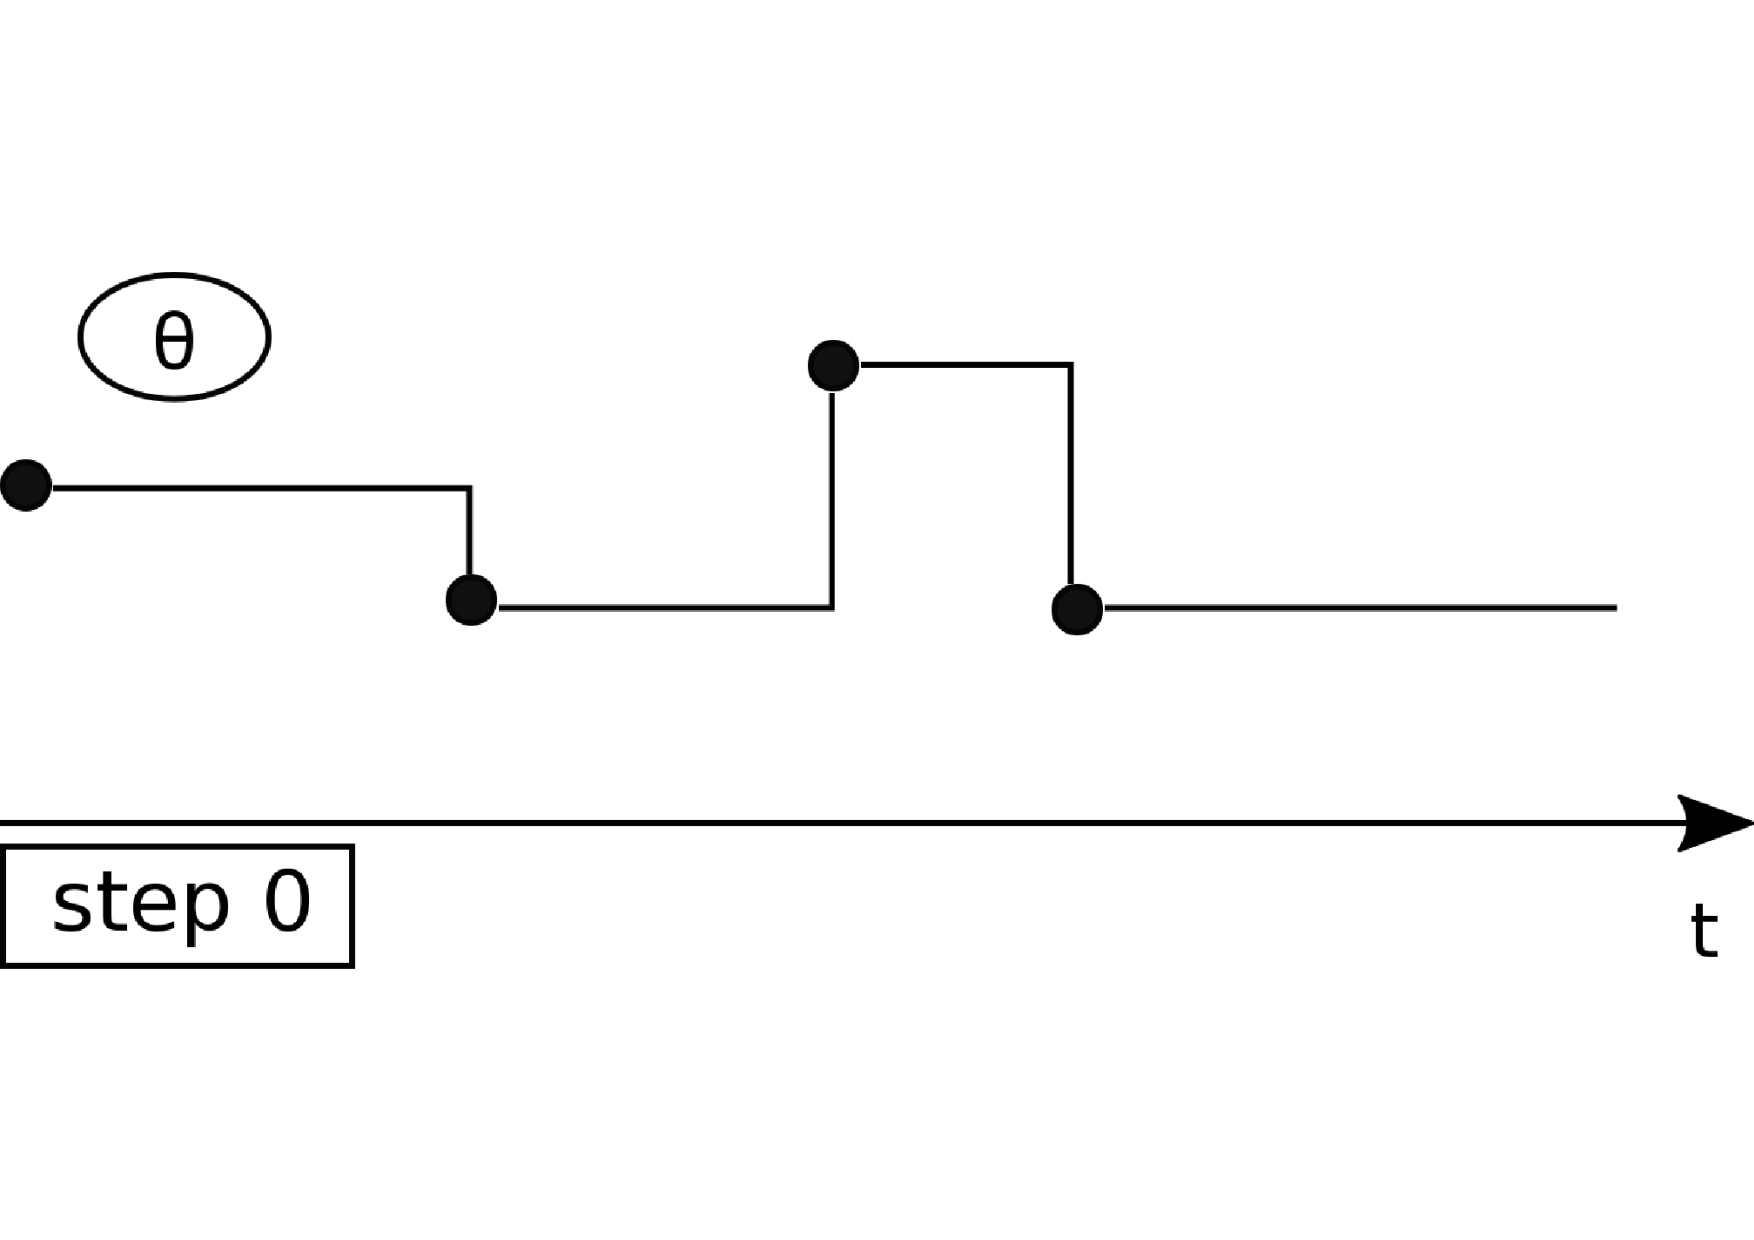
\includegraphics [width=0.70\textwidth, angle=0]{figs/plotn0.pdf}
      \end{minipage}
  \begin{minipage}[!hp]{0.45\linewidth}
  \centering
    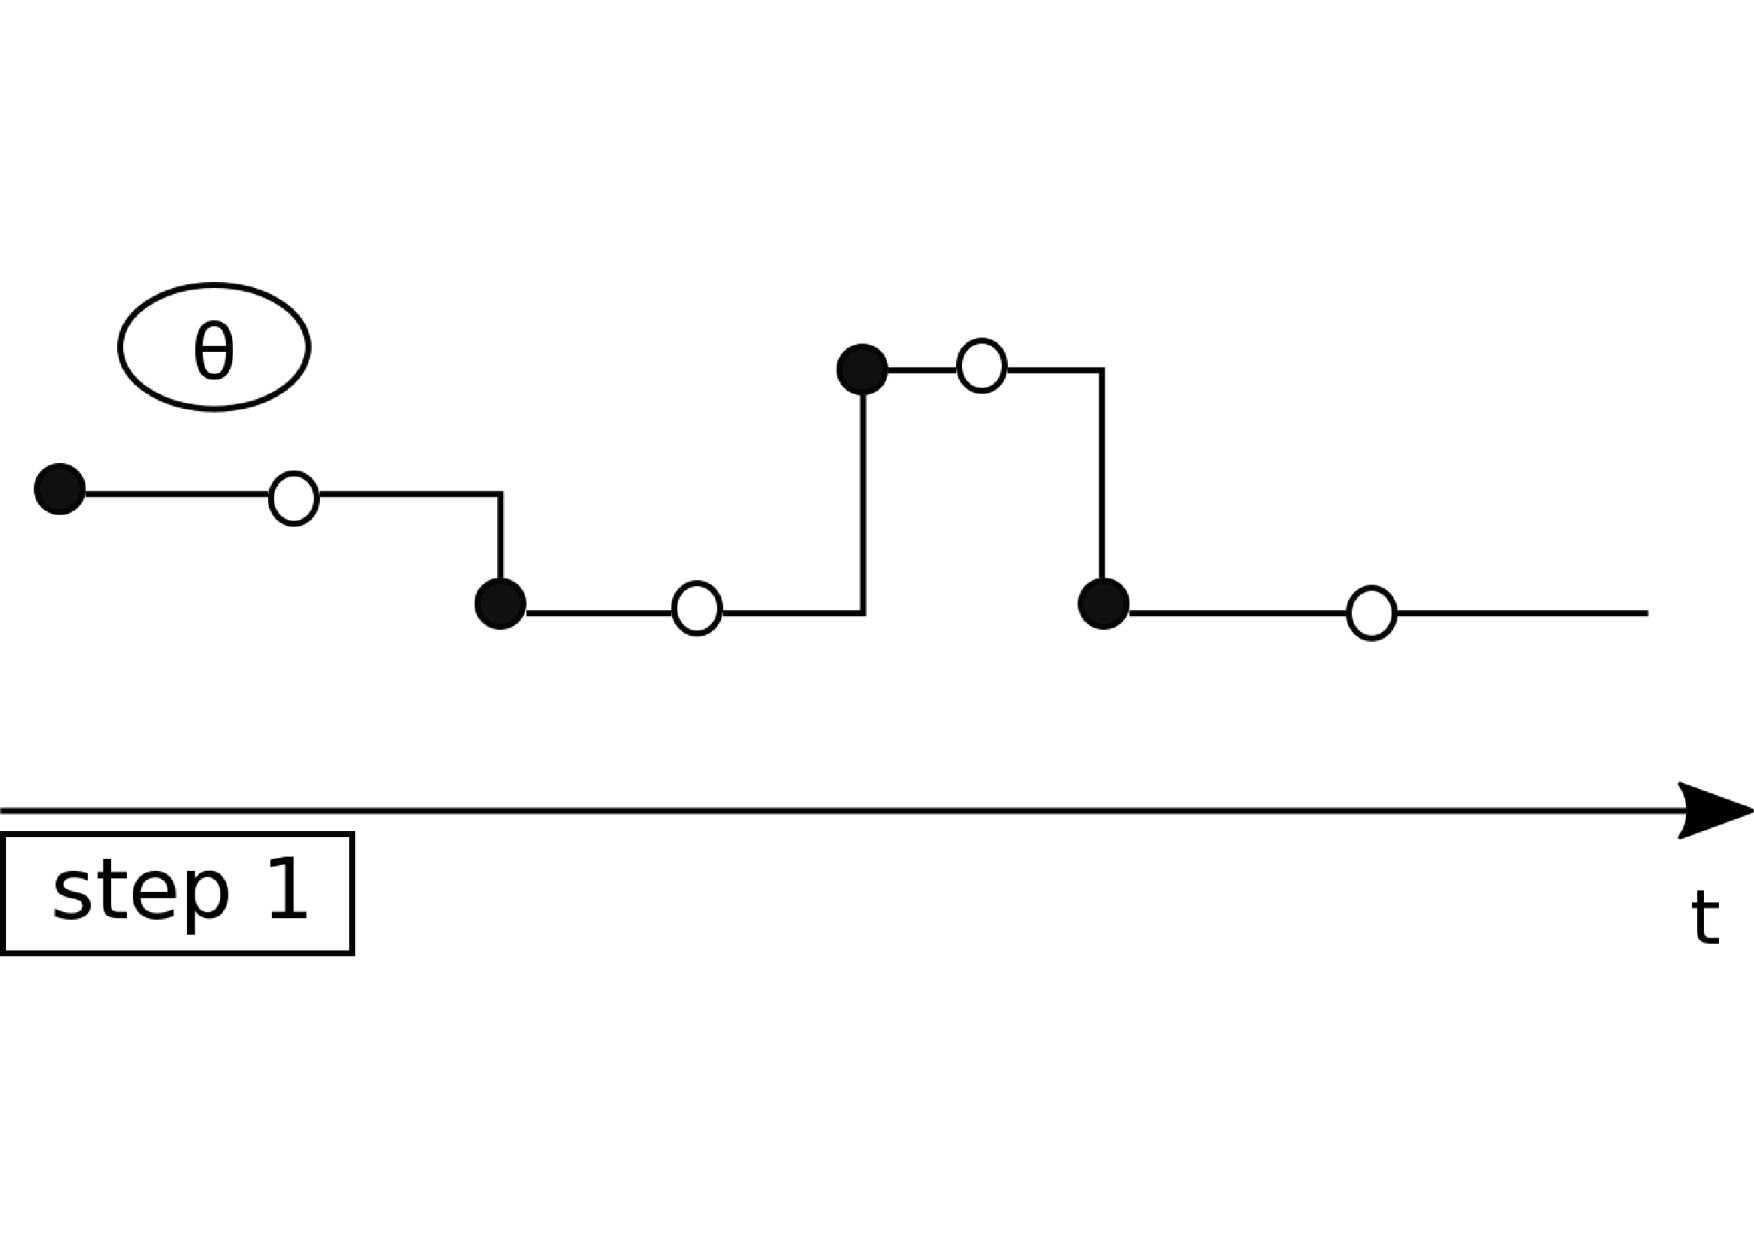
\includegraphics [width=0.70\textwidth, angle=0]{figs/plotn1.pdf}
    \vspace{-0 in}
  \end{minipage}
  \begin{minipage}[!hp]{0.45\linewidth}
  \centering
    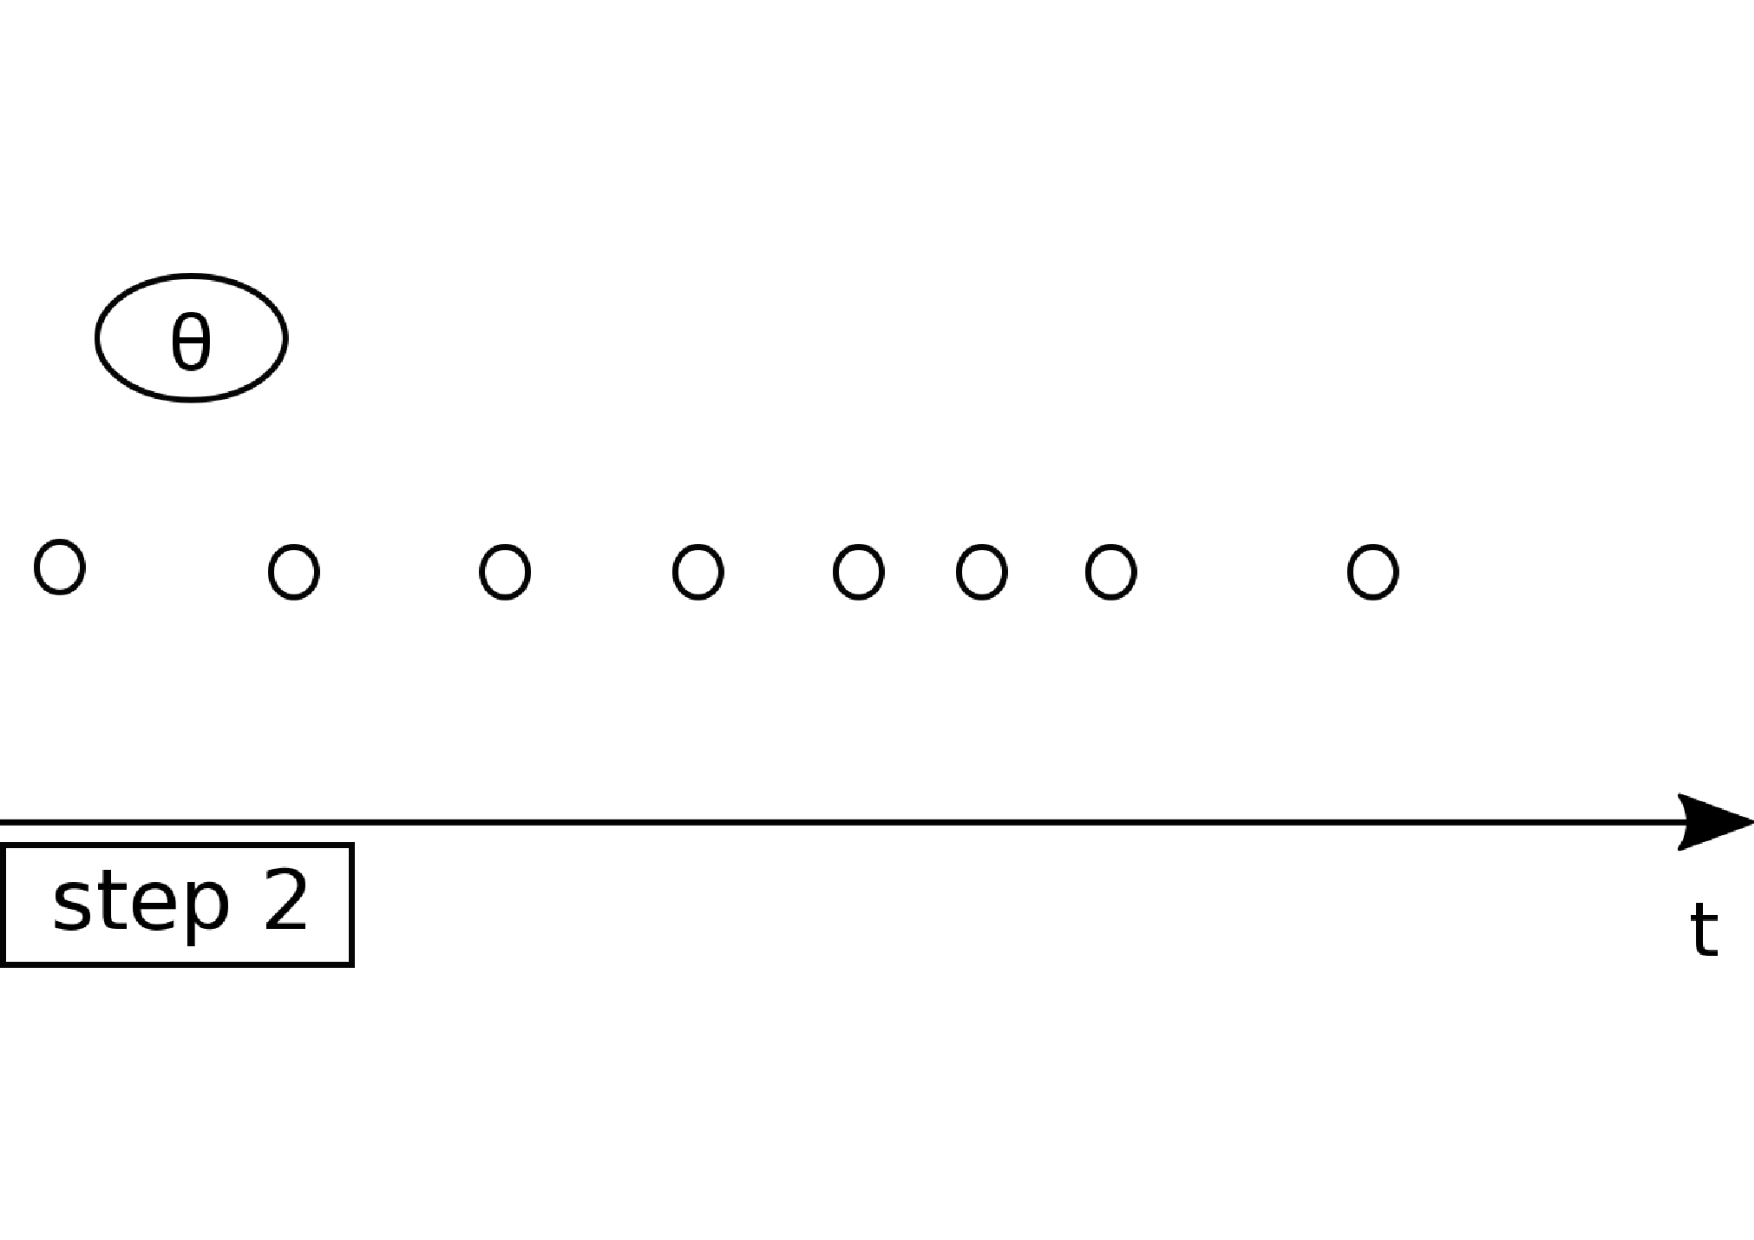
\includegraphics [width=0.70\textwidth, angle=0]{figs/plotn2.pdf}
    \vspace{-0 in}
  \end{minipage}
  \begin{minipage}[!hp]{0.45\linewidth}
  \centering
    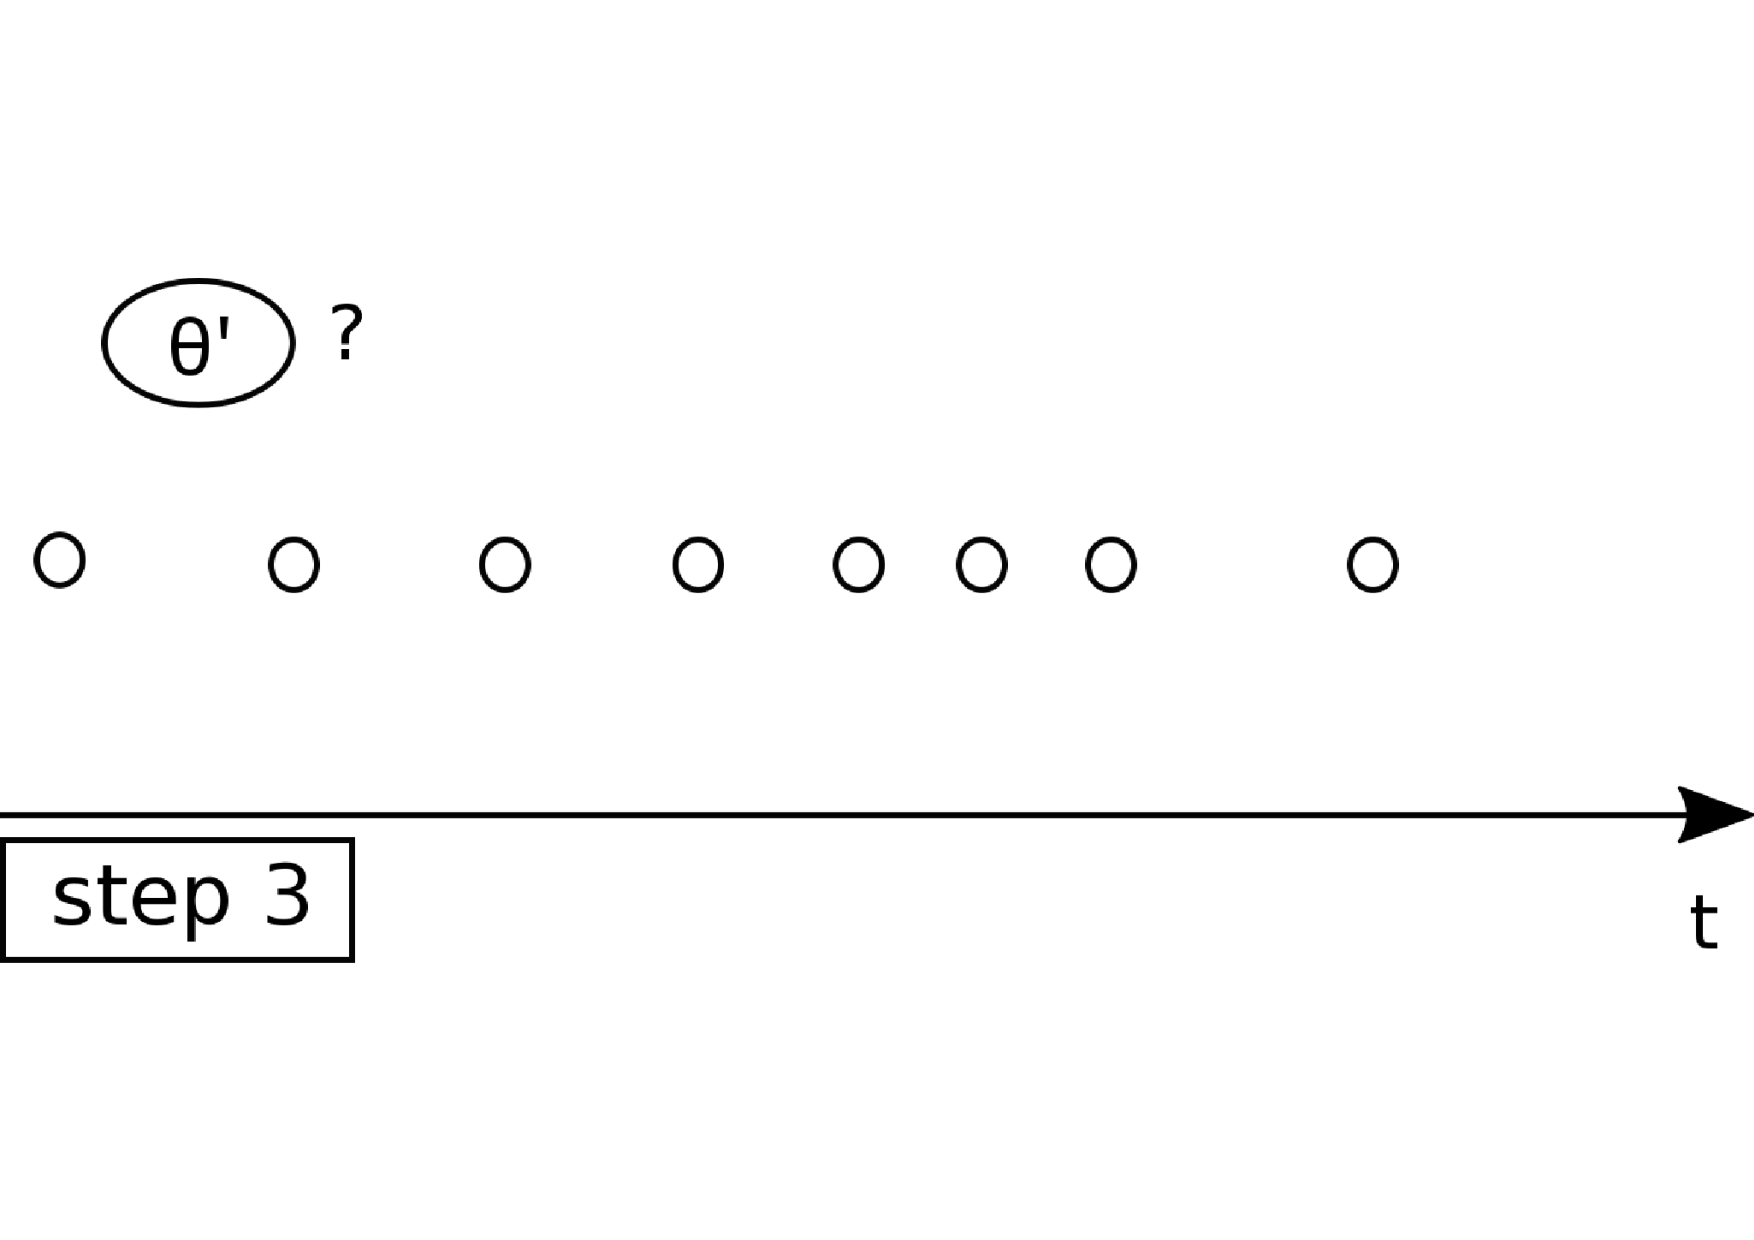
\includegraphics [width=0.70\textwidth, angle=0]{figs/plotn3.pdf}
    \vspace{-0 in}
  \end{minipage}
  \begin{minipage}[!hp]{0.45\linewidth}
  \centering
    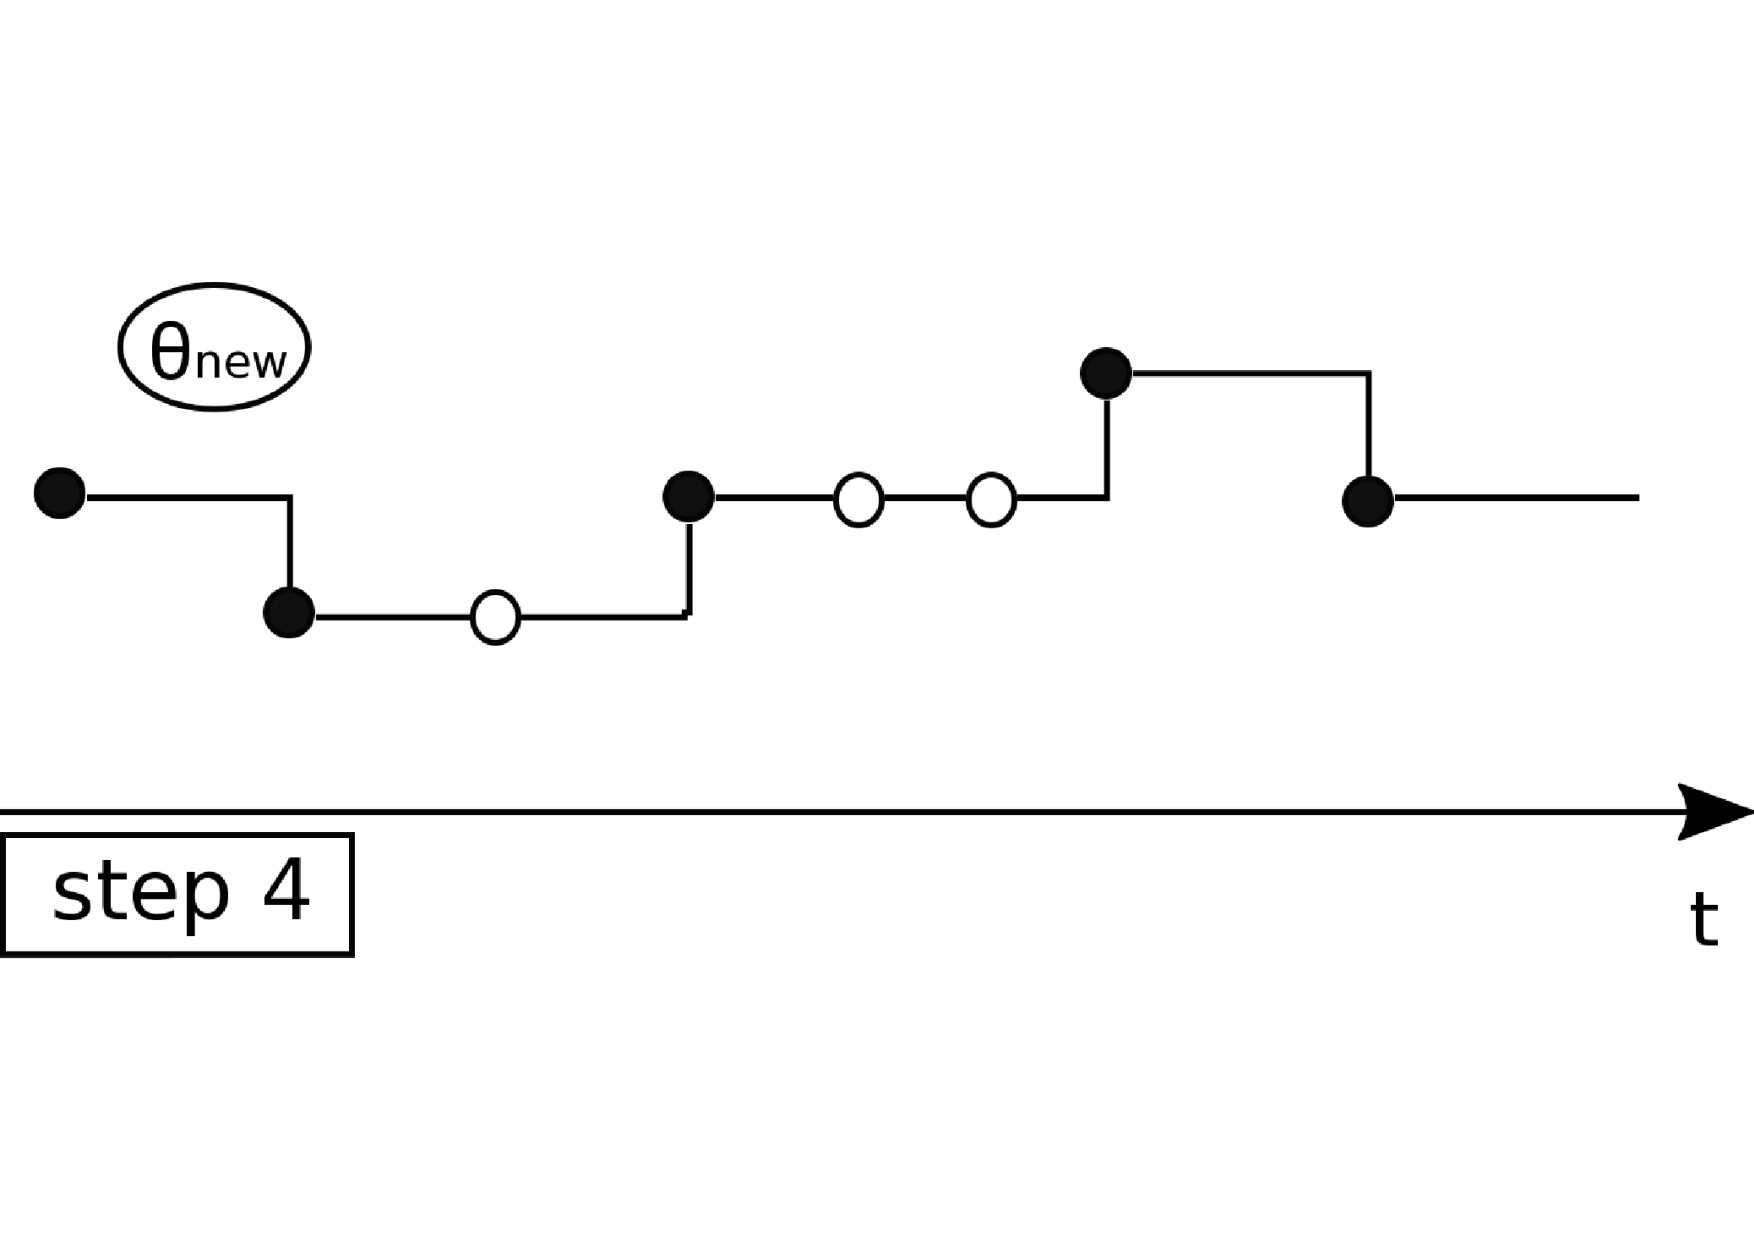
\includegraphics [width=0.70\textwidth, angle=0]{figs/plotn4.pdf}
    \vspace{-0 in}
  \end{minipage}
  \begin{minipage}[!hp]{0.45\linewidth}
  \centering
    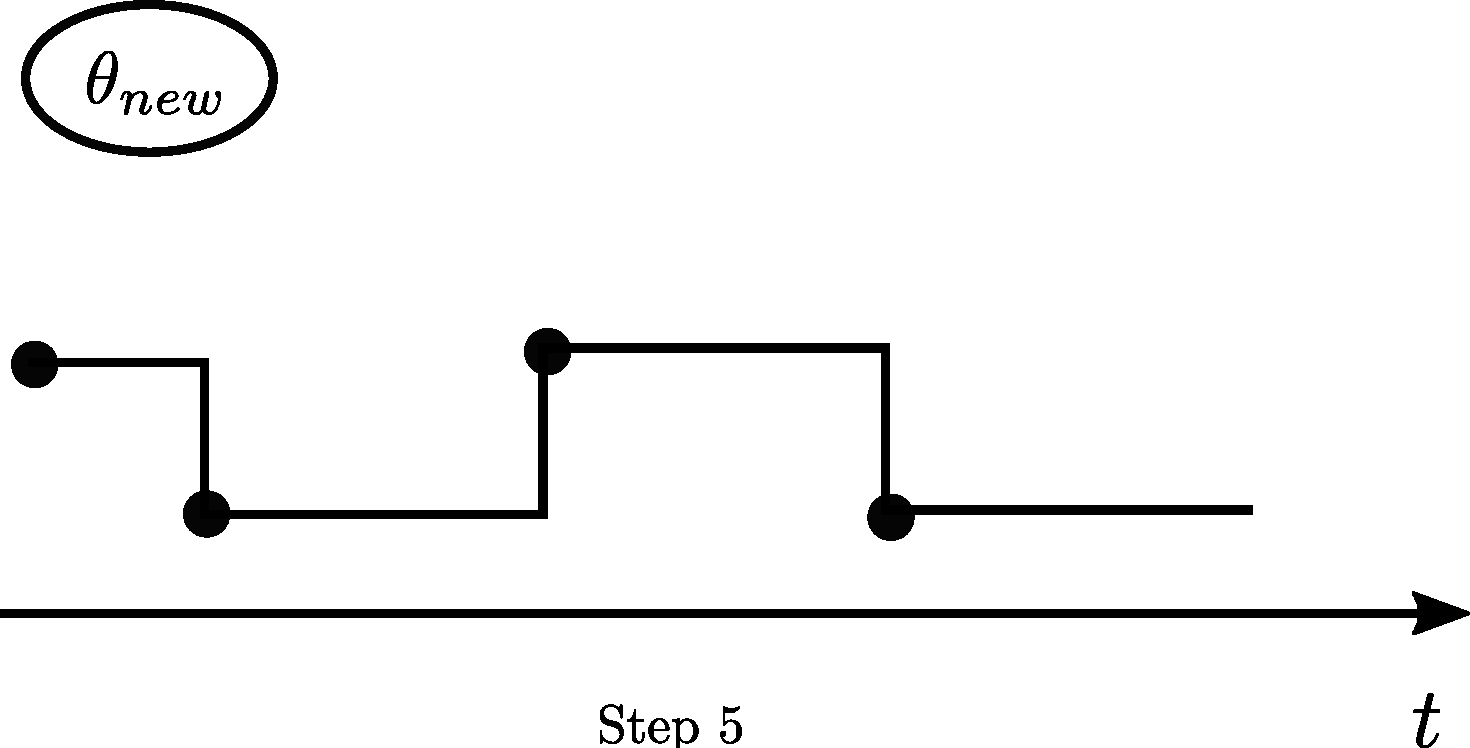
\includegraphics [width=0.70\textwidth, angle=0]{figs/plotn5.pdf}
    \vspace{-0 in}
  \end{minipage}
  \caption{\Naive\ MH-algorithm: Step 0 to 2: sample thinned events
  and discard state information to get a random grid. Step 3: 
propose a new parameter $\theta'$, and accept or reject by making
a forward pass on the grid. Steps 4 to 5: make a backward pass using
the accepted parameter and discard self-transitions to produce a new
trajectory.}
   \label{fig:naive_mh}
  \end{figure}

\subsection{Additional results}
In the following, we evaluate Python implementations of a number of algorithms, including the \naive\ MH algorithm (Algorithm~\ref{alg:MH_naive}, which we plot in yellow), and our main contribution, the symmetrized MH algorithm (algorithm~\ref{alg:MH_improved}, plotted as dashed red lines\vinayak{Do this}). 
We compare different variants of these algorithms, corresponding to different uniformizing Poisson rates. % (i.e.\ different choices of $\kappa$, see section~\ref{sec:comments}). 
For \naive\ MH, we set $\Omega(\theta) = \kappa \max_s A_s(\theta) $ with $\kappa$  equal to $1.5, 2$ and $3$, represented in our plots with circles, triangles and square symbols. 
For symmetrized MH, where the uniformizing rate depends on both the current and proposed parameter, we consider two settings:
 $\Omega(\theta, \vartheta) = \kappa (\max A(\theta) + \max A(\vartheta))$ 
 ($\kappa = 1$ and $1.5$, plotted with {triangles} and {squares}), and 
$\Omega(\theta, \vartheta) = \kappa \max(\max A(\theta), \max A(\vartheta))$
($\kappa=1.5$, plotted with {circles}).  
We also evaluate two baselines: Gibbs sampling (Algorithm~\ref{alg:MJP_gibbs}, plotted in blue), and particle MCMC~\citep{Andrieu10}, plotted in black. 
Gibbs sampling involves a uniformization step to update the MJP trajectory, for which we used three settings, $\kappa=1.5,2,3$, plotted with circles, {triangles} and {squares}.  
Unless specified, our results were obtained from $100$ independent MCMC runs, each of $10000$ iterations.
We found particle MCMC to be more computationally intensive, and limited each run to $3000$ iterations, the number of particles being $5, 10$ and $20$ (plotted with circles, trianges and squares). 

\vspace{-.4in}
  \begin{figure}[H]
  \centering
  \begin{minipage}[h!]{0.65\linewidth}
  \centering
    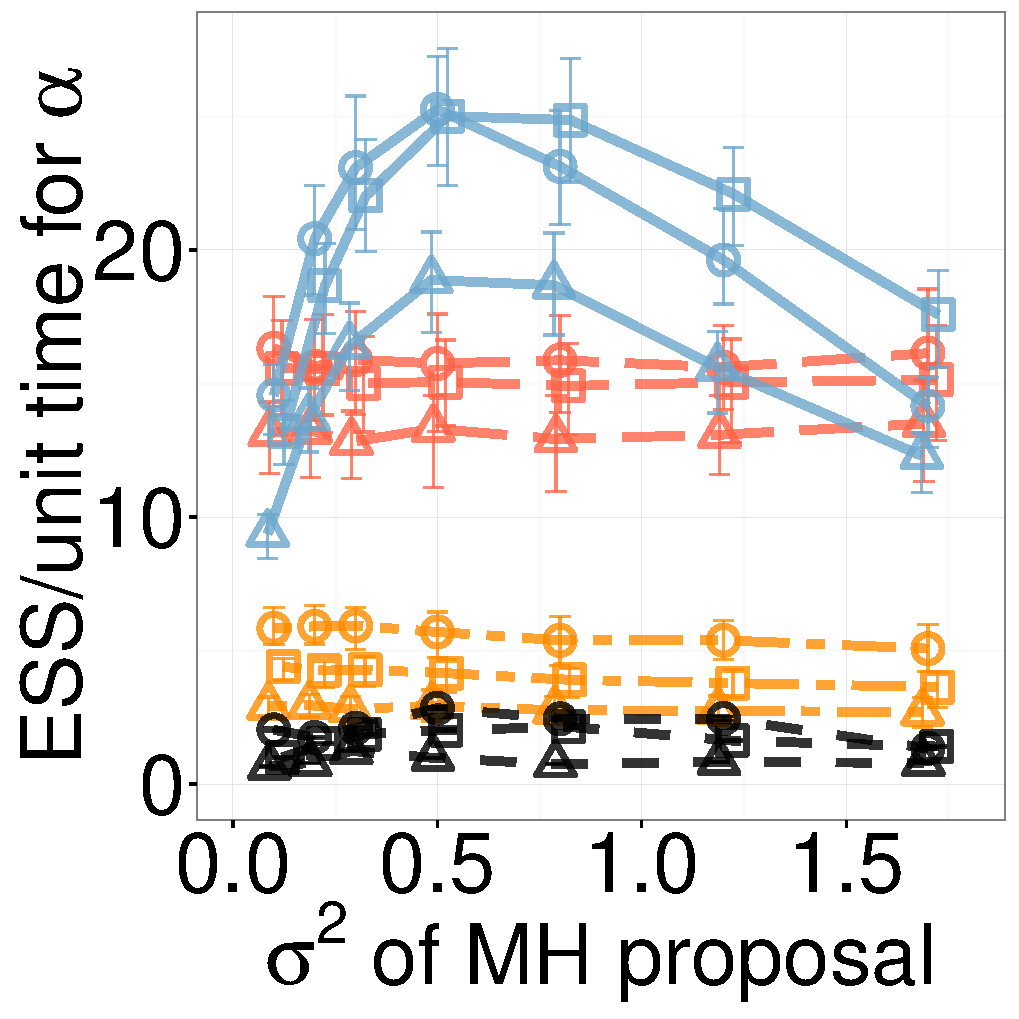
\includegraphics [width=0.44\textwidth, angle=0]{figs/new_whole_exp_figs/exp_alpha_dim3.pdf}
    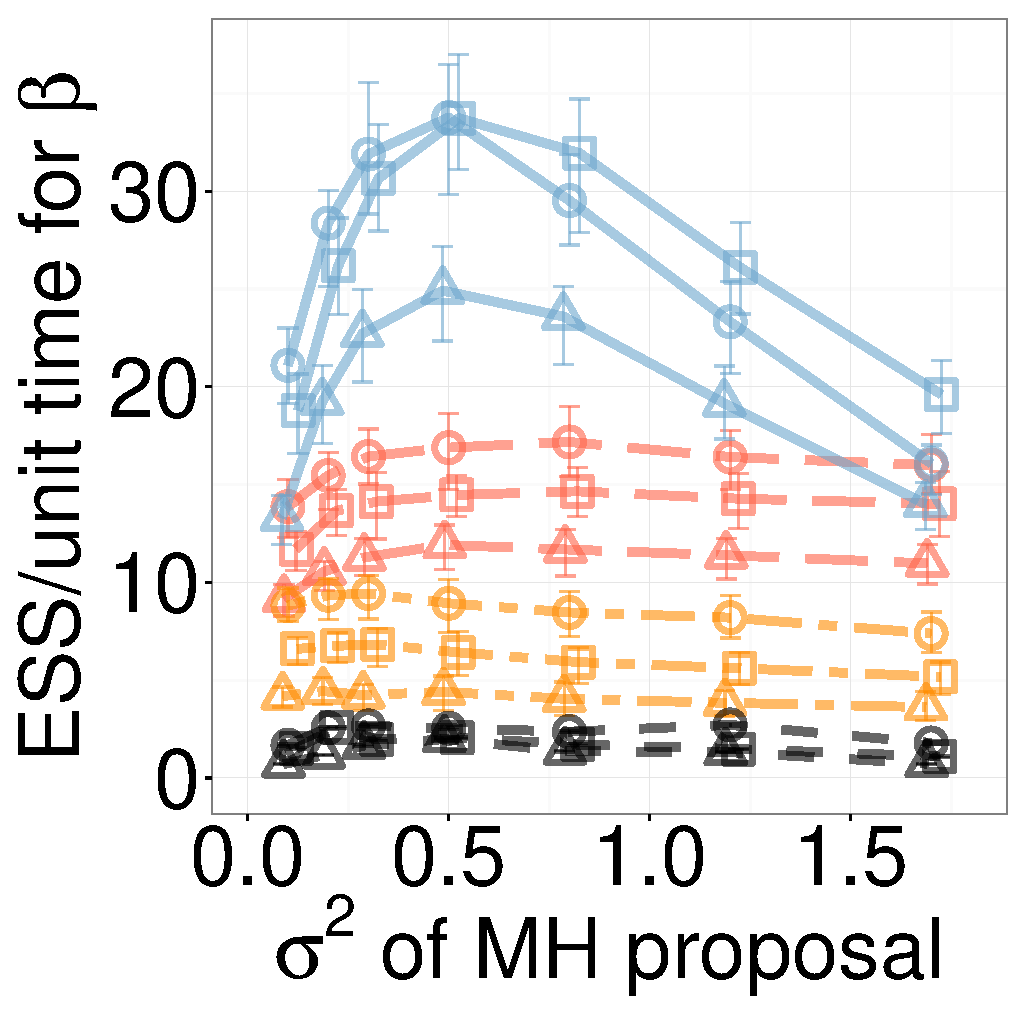
\includegraphics [width=0.44\textwidth, angle=0]{figs/new_whole_exp_figs/exp_beta_dim3.pdf}
  \end{minipage}
  \begin{minipage}[!hp]{0.33\linewidth}
    \caption{ESS/sec for the synthetic  model, dimension 3. (Left, right) 
      are $(\alpha, \beta)$. Blue, yellow, red and black are the symmetrized MH,
  \naive\ MH, Gibbs and particle MCMC algorithm. Different symbols are
different settings of the algorithms, see section~\ref{sec:expts}.}
     \label{fig:ESS_EXP_D33}
  \end{minipage}
  \end{figure}

\vspace{-.4in}
  \begin{figure}[H]
  \centering
  \begin{minipage}[h!]{0.65\linewidth}
  \centering
    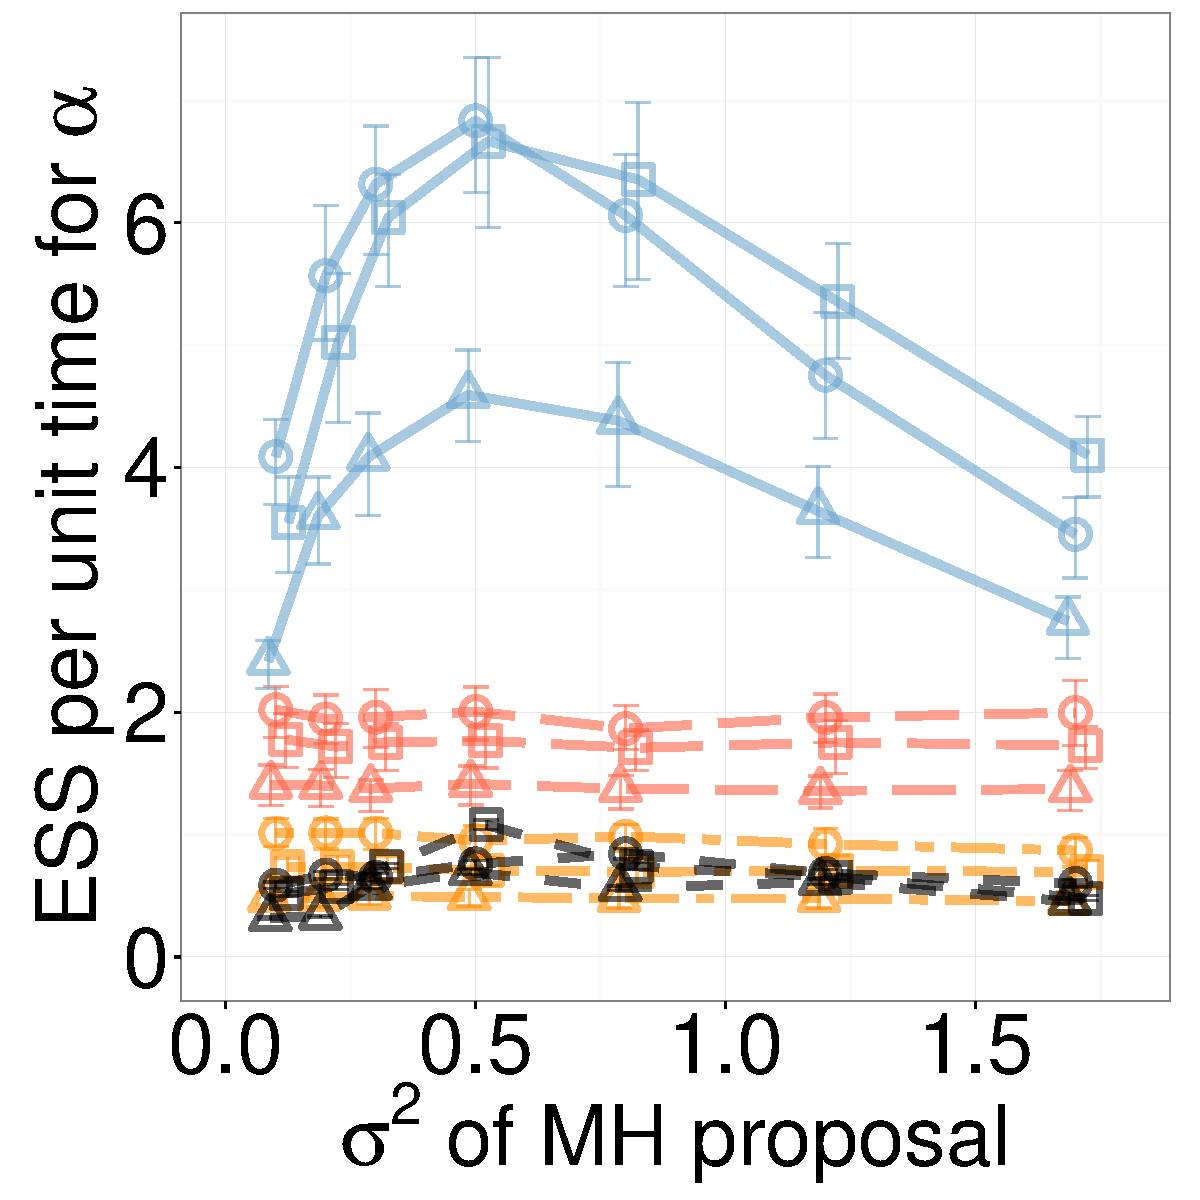
\includegraphics [width=0.44\textwidth, angle=0]{figs/new_whole_exp_figs/exp_alpha_dim5.pdf}
    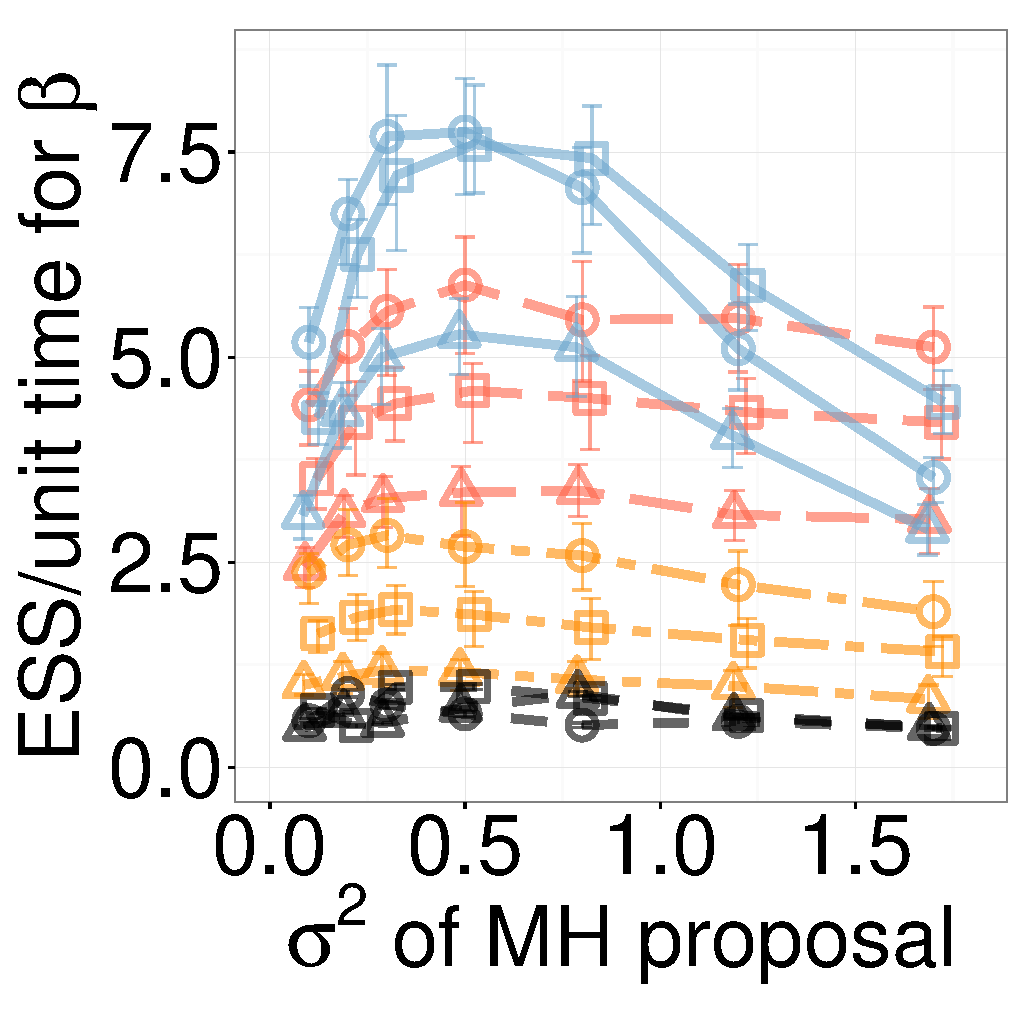
\includegraphics [width=0.44\textwidth, angle=0]{figs/new_whole_exp_figs/exp_beta_dim5.pdf}
  \end{minipage}
  \begin{minipage}[!hp]{0.33\linewidth}
    \caption{ESS/sec for the synthetic  model, dimension 5. (Left, right) 
      are $(\alpha, \beta)$. Blue, yellow, red and black are the symmetrized MH,
  \naive\ MH, Gibbs and particle MCMC algorithm. Different symbols are
different settings of the algorithms, see section~\ref{sec:expts}.}
     \label{fig:ESS_EXP_D55}
  \end{minipage}
  \end{figure}
  %\centering
\vspace{-.4in}
\vspace{-.4in}
  \begin{figure}[H]
  \centering
  \begin{minipage}[h!]{0.65\linewidth}
  \centering
    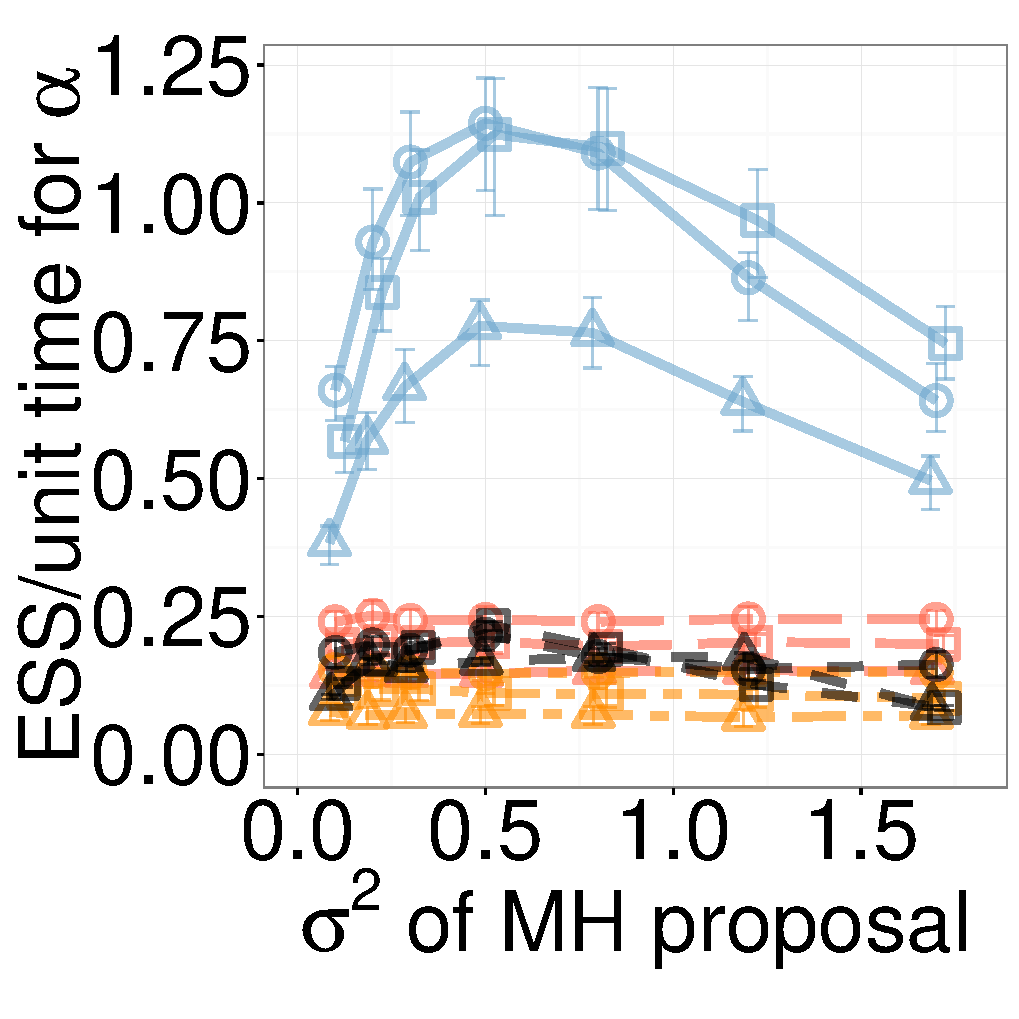
\includegraphics [width=0.44\textwidth, angle=0]{figs/new_whole_exp_figs/exp_alpha_dim10.pdf}
    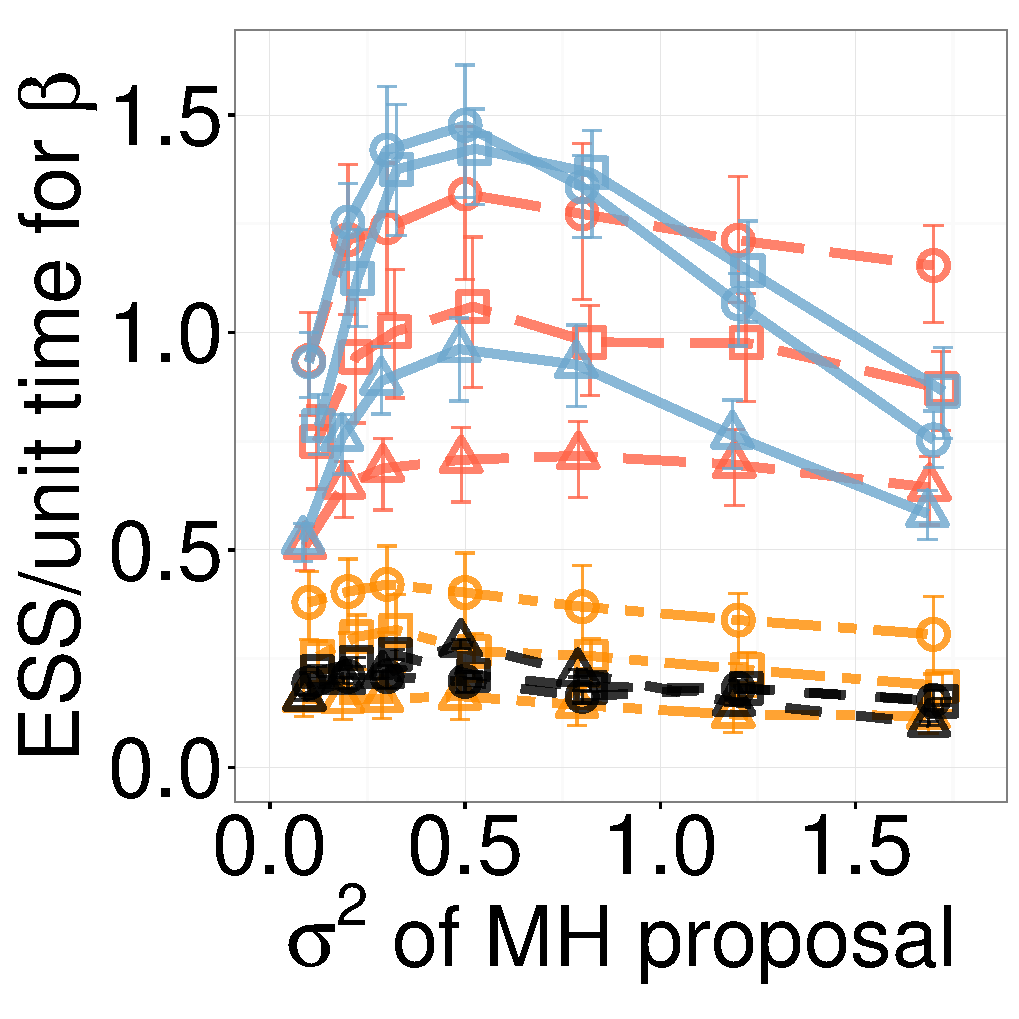
\includegraphics [width=0.44\textwidth, angle=0]{figs/new_whole_exp_figs/exp_beta_dim10.pdf}
  \end{minipage}
  \begin{minipage}[!hp]{0.33\linewidth}
    \caption{ESS/sec for the synthetic  model, dimension 10. (Left, right) 
      are $(\alpha, \beta)$. Blue, yellow, red and black are the symmetrized MH,
  \naive\ MH, Gibbs and particle MCMC algorithm. Different symbols are
different settings of the algorithms, see section~\ref{sec:expts}.}
     \label{fig:ESS_EXP_D1010}
  \end{minipage}
  \end{figure}

  \begin{figure}[H]
%    \vspace{-.2in}
  \centering

  \begin{minipage}[!hp]{0.99\linewidth}
    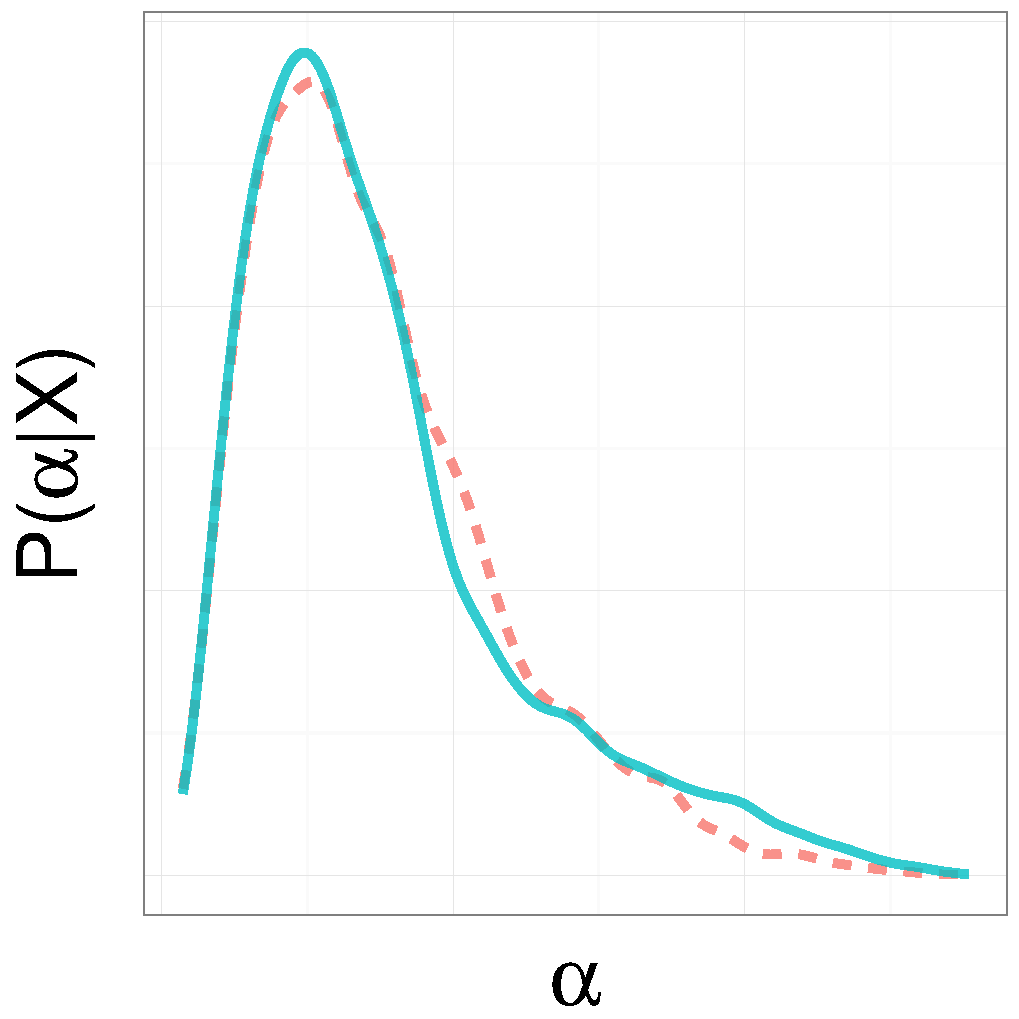
\includegraphics [width=0.3\textwidth, angle=0]{figs/EXP_ks/exp_hist_44_05_10_.pdf}
    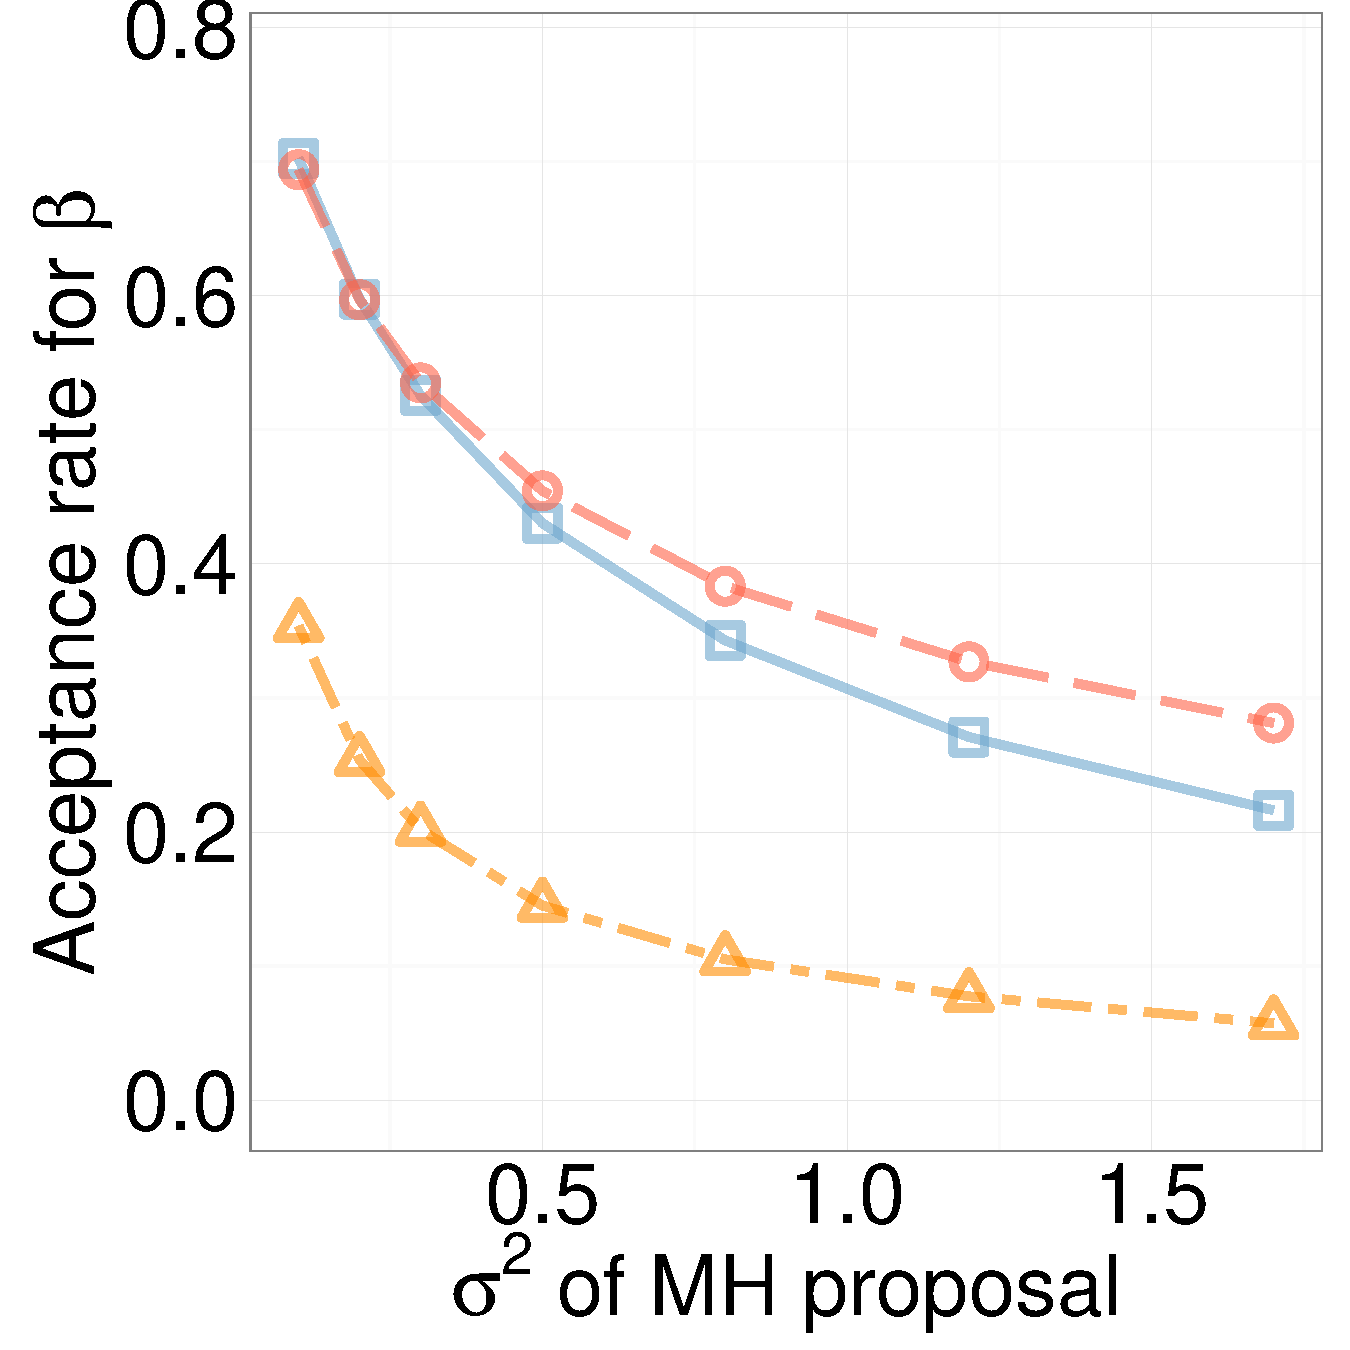
\includegraphics [width=0.30\textwidth, angle=0]{figs/acc/EXP_D3beta_k2.pdf}
	\hspace{.5in}
    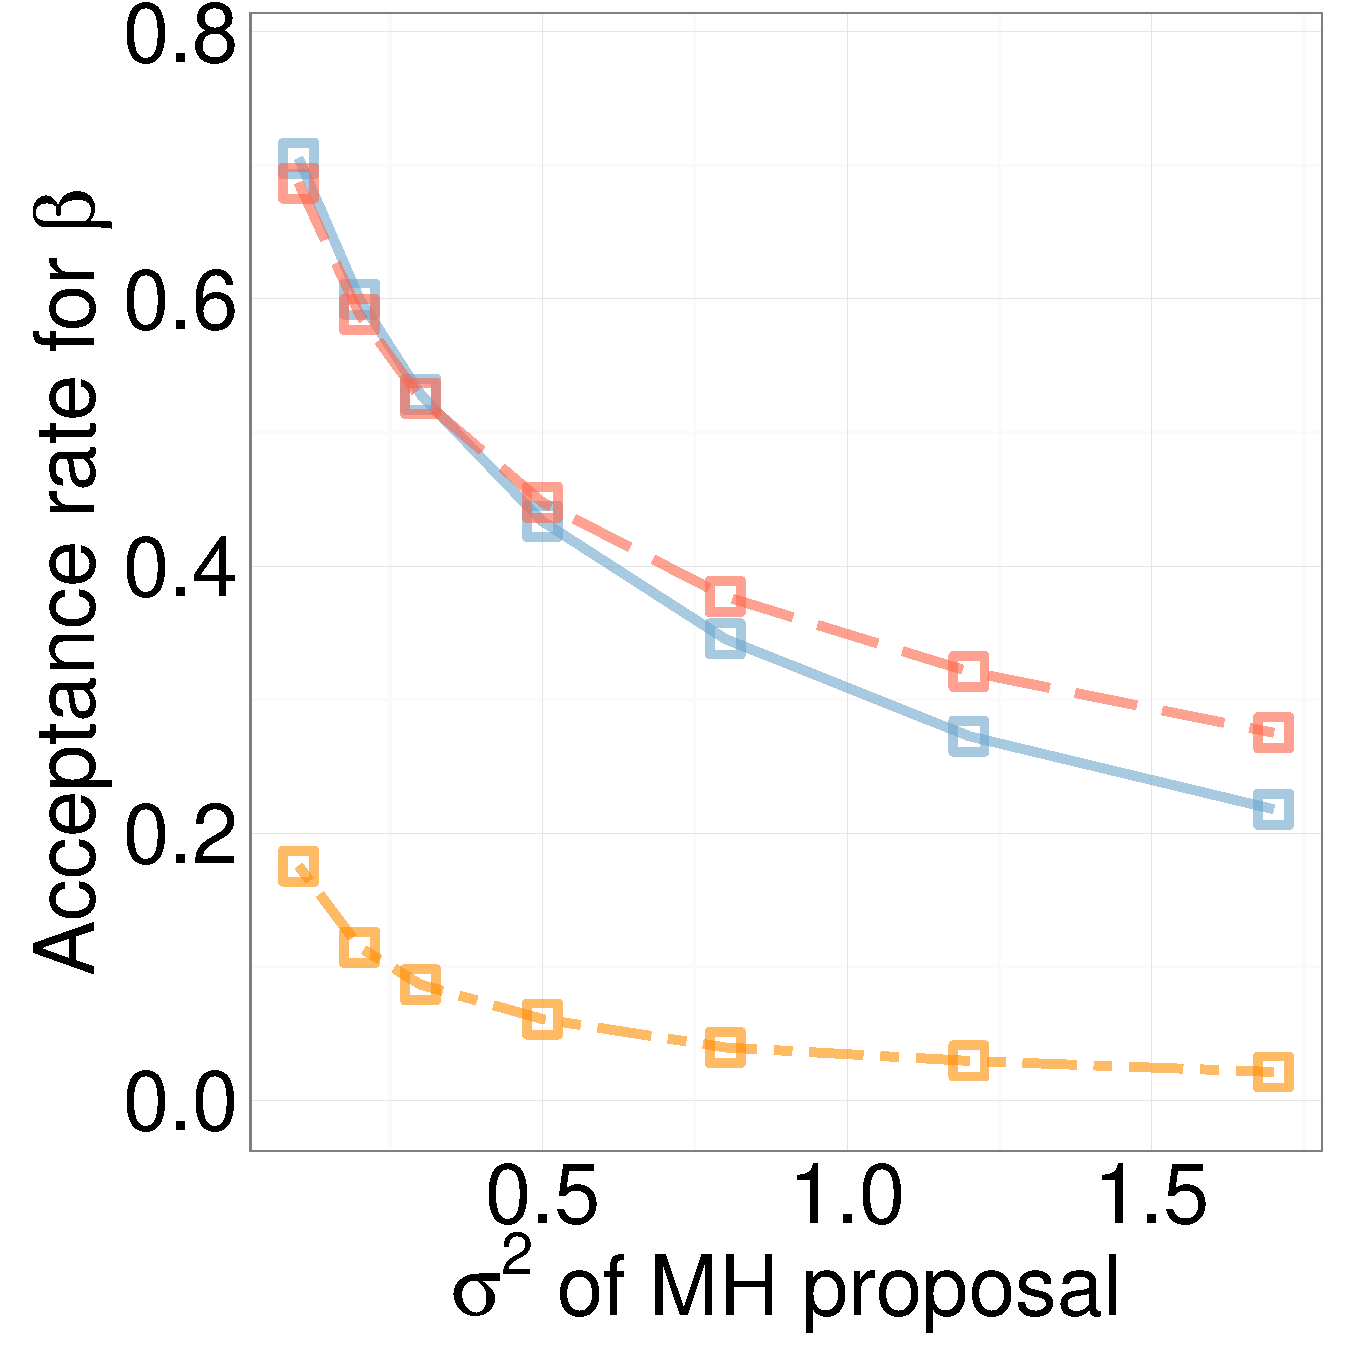
\includegraphics [width=0.30\textwidth, angle=0]{figs/acc/EXP_D10beta_k2.pdf}
  \end{minipage}
%  \begin{minipage}[!hp]{0.99\linewidth}
    \caption{Acceptance Rate for $\beta$ in the synthetic model, the left row being dimension 3, and the right,dimension 10.  Red, yellow and blue curves are the Gibbs, symmetrized MH,
 and \naive\ MH  algorithm. The multiplicative factor is $2$. }
     \label{fig:ACC_EXP}
%  \end{minipage}
  \end{figure}
  \begin{figure}[H]
%    \vspace{-.2in}
  \centering

  \begin{minipage}[!hp]{0.99\linewidth}
  	\centering
    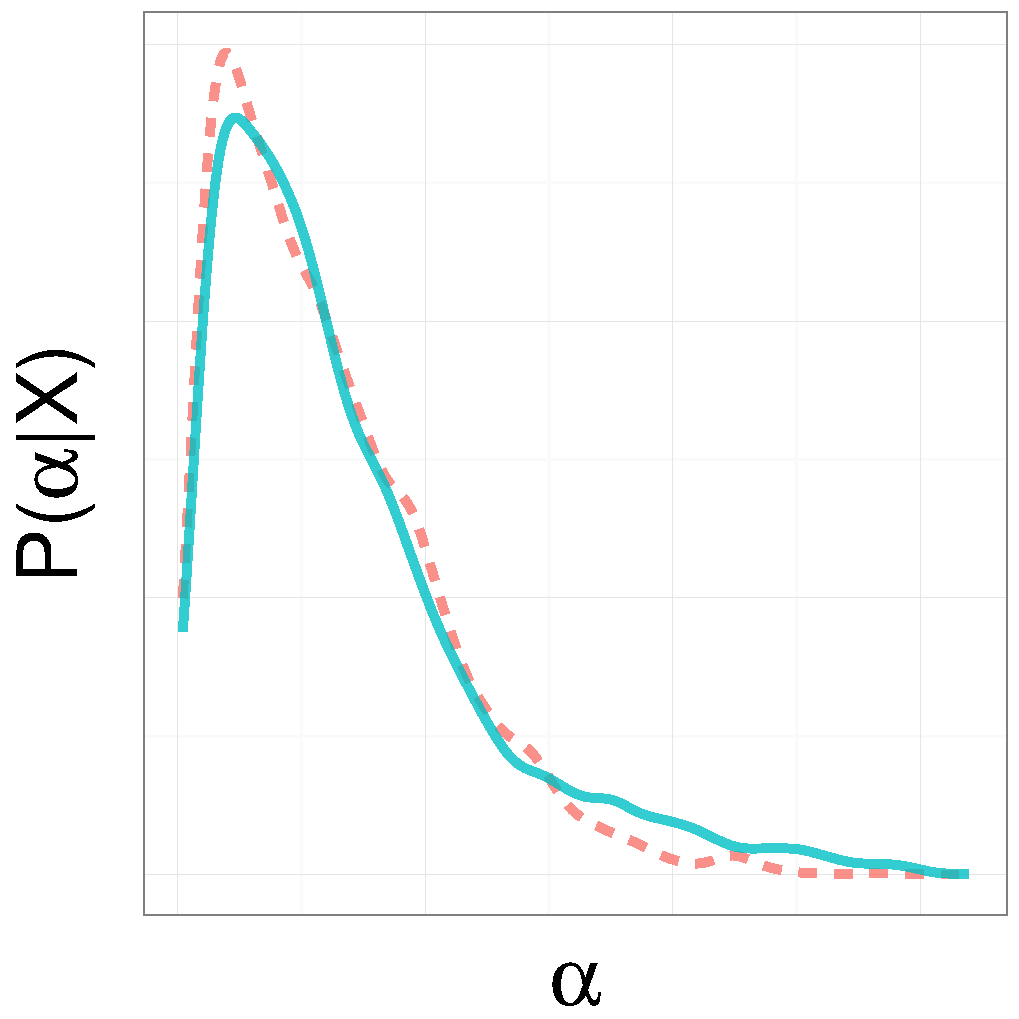
\includegraphics [width=0.3\textwidth, angle=0]{figs/JC_ks/jc_hist_44_05_3_.pdf}
    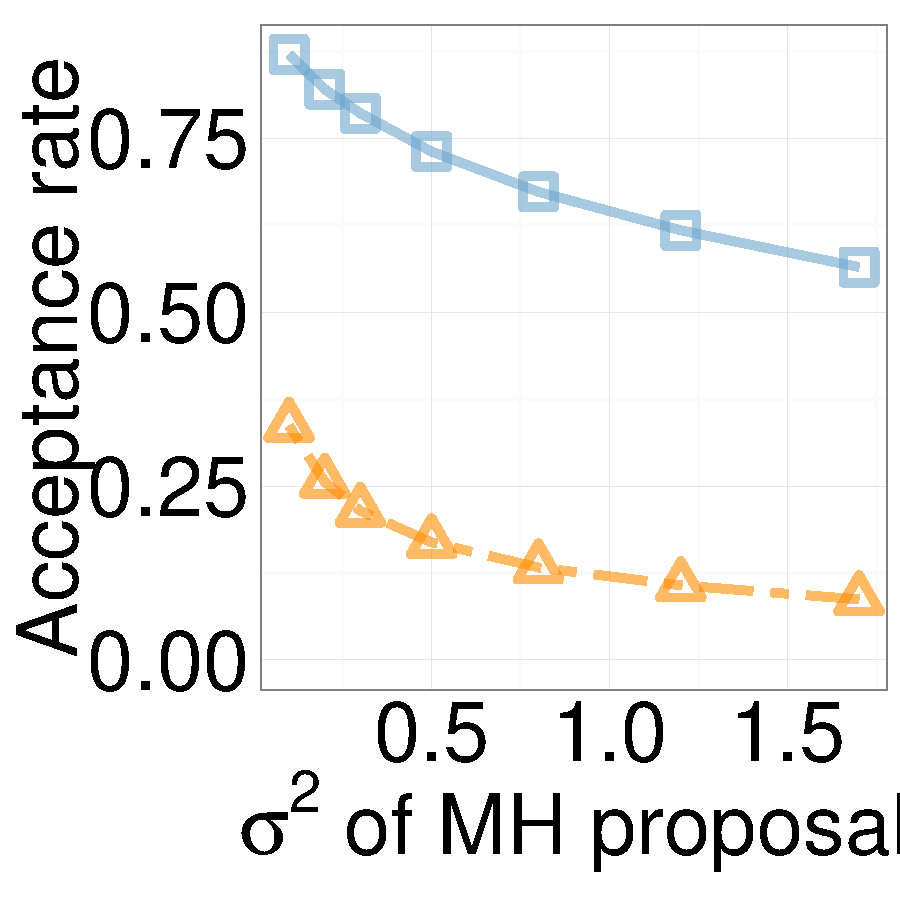
\includegraphics [width=0.3\textwidth, angle=0]{figs/acc/JCalpha_k2.pdf}
	\hspace{.5in}
    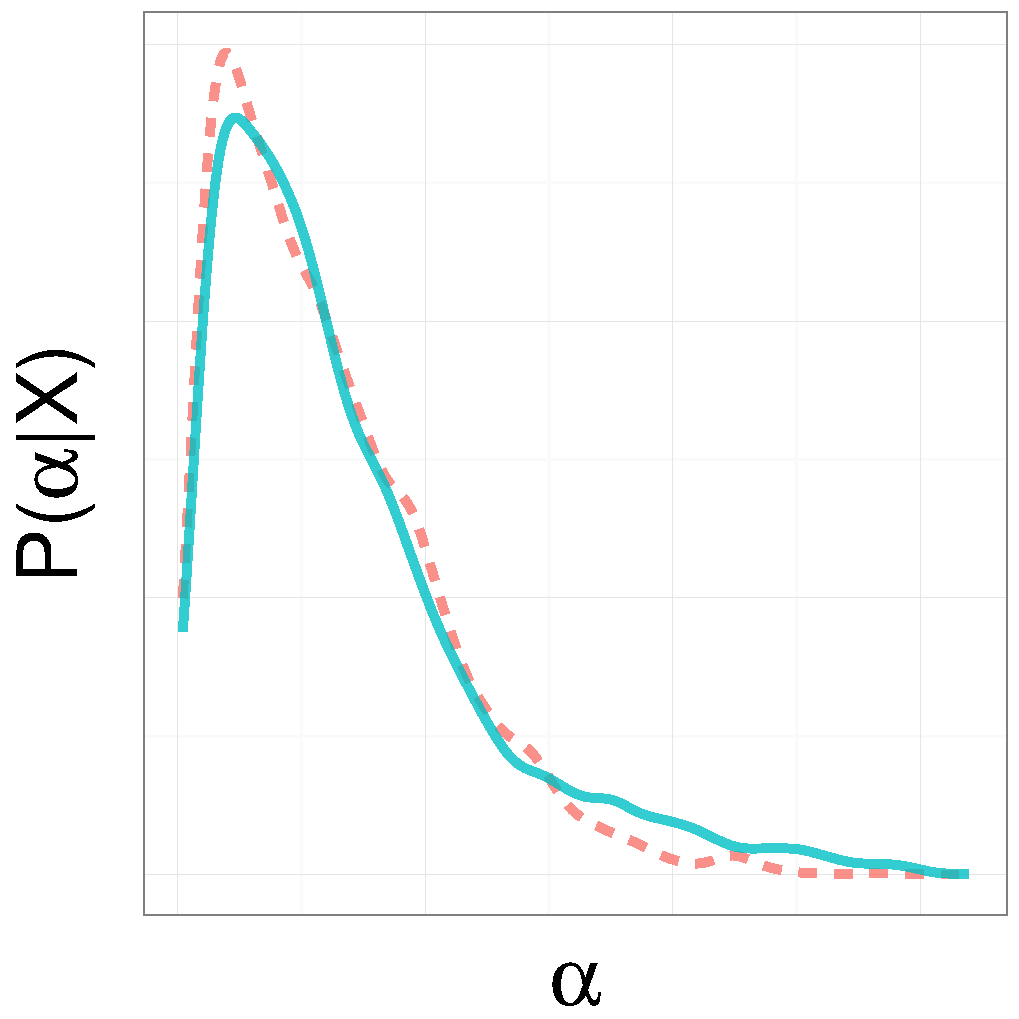
\includegraphics [width=0.3\textwidth, angle=0]{figs/JC_ks/jc_hist_44_05_3_.pdf}
  \end{minipage}
%  \begin{minipage}[!hp]{0.99\linewidth}
    \caption{The left represents the acceptance rate for $\alpha$ in the JC69 model.  Yellow and blue curves represent symmetrized MH,and \naive\ MH  algorithm. The multiplicative factor is $2$.The right is histogram for the posterior samples($\alpha$ ) of the JC69 model, the red and blue curves are the Gibbs and symmetrized MH. The p value of the two sample-Kolmogorov Smirnov test is $ 0.97$.  }
     \label{fig:ACC_JC}
%  \end{minipage}
  \end{figure}
  
  \begin{figure}[H]
%    \vspace{-.2in}
  \centering
%  \begin{minipage}[!hp]{0.99\linewidth}
 % \centering
  \begin{minipage}[!hp]{0.99\linewidth}
    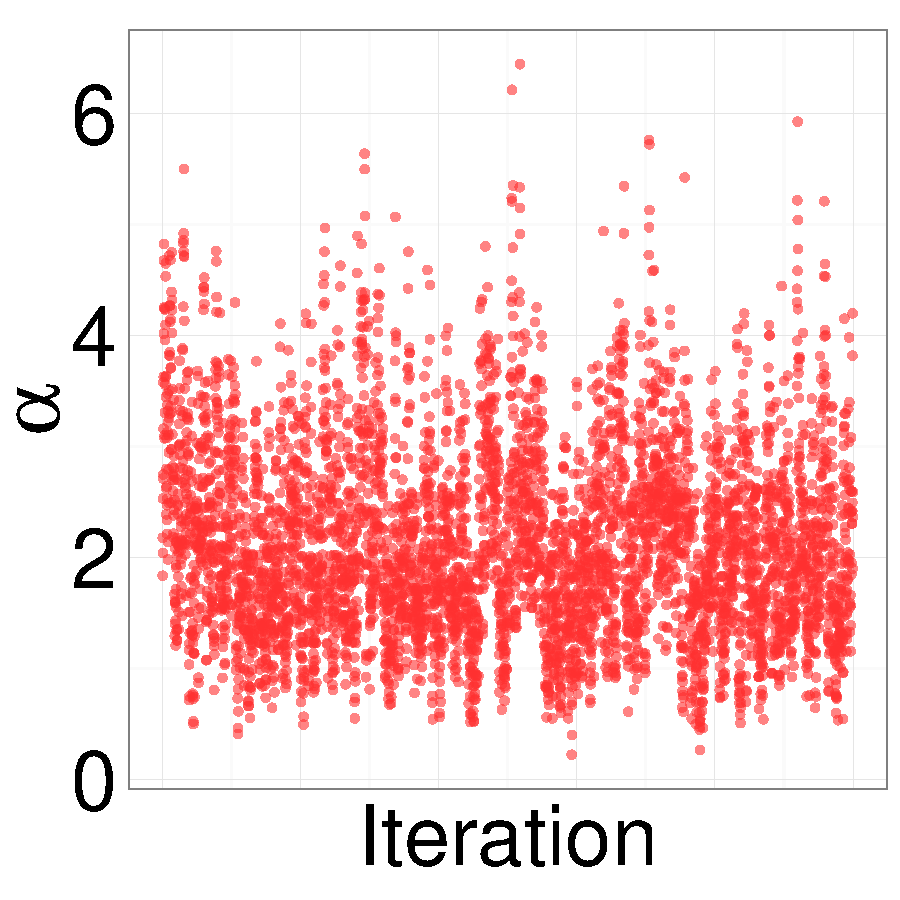
\includegraphics [width=0.24\textwidth, angle=0]{figs/Q_ks/q_traceGBS_20_03_3_.pdf}
    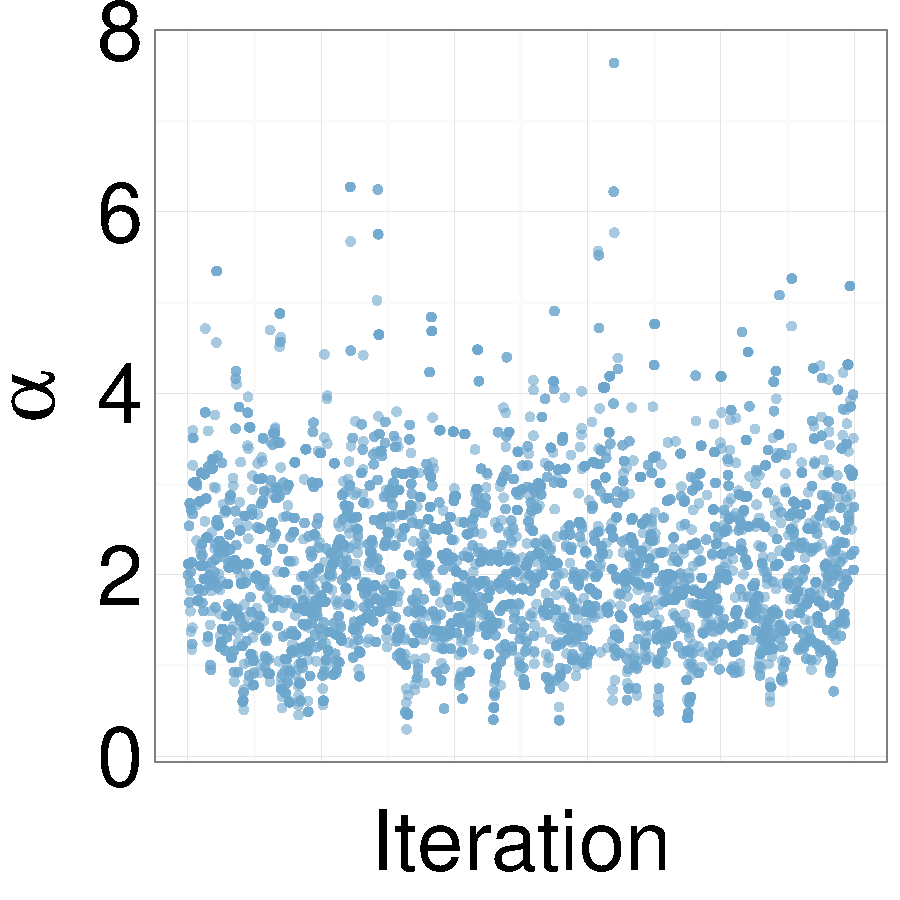
\includegraphics [width=0.24\textwidth, angle=0]{figs/Q_ks/q_traceMH_20_03_3_.pdf}
    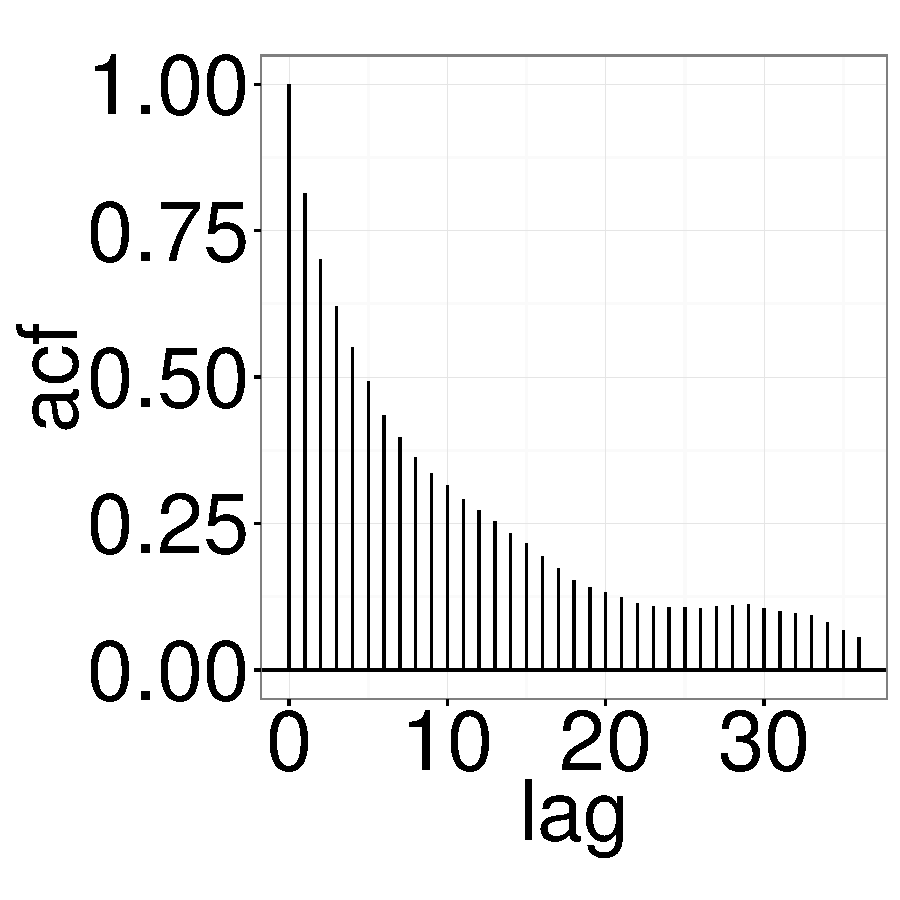
\includegraphics [width=0.24\textwidth, angle=0]{figs/Q_ks/q_gbsacf_20_03_3_.pdf}
    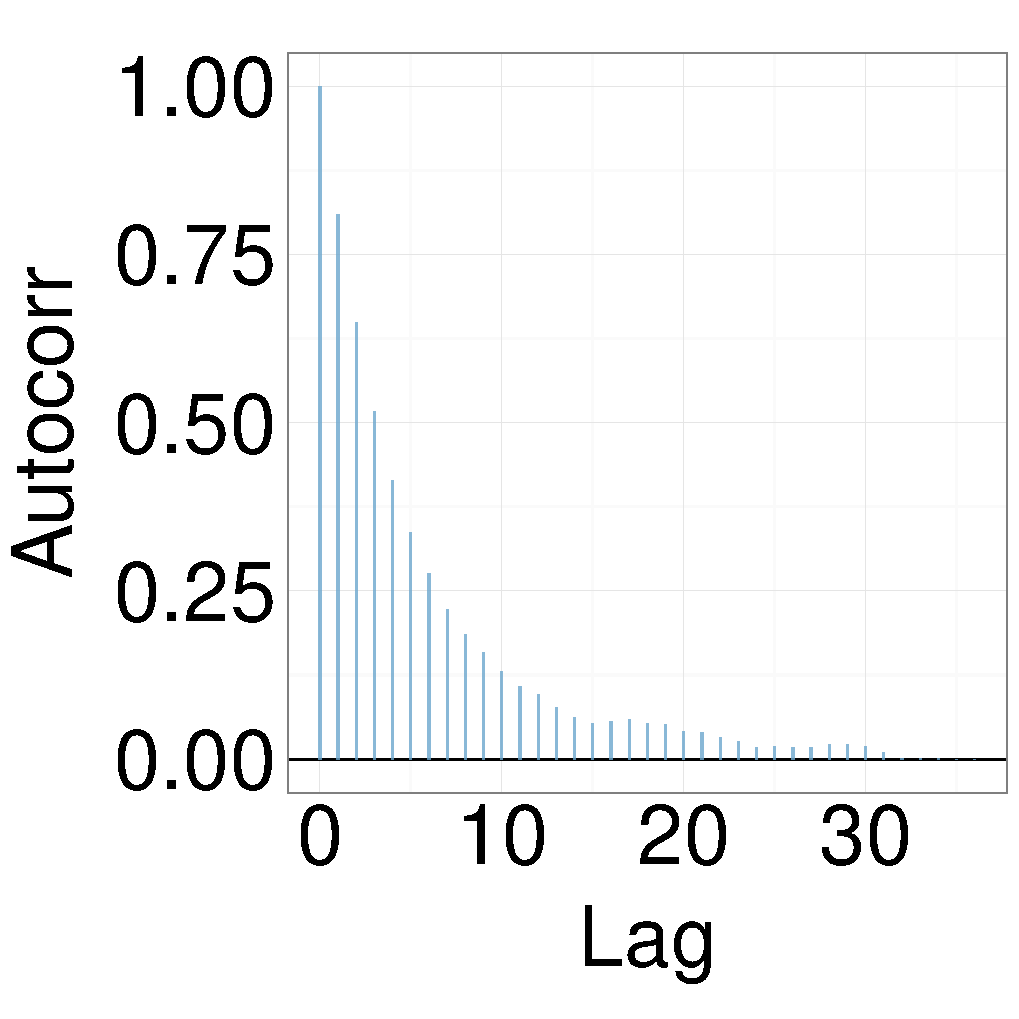
\includegraphics [width=0.24\textwidth, angle=0]{figs/Q_ks/q_mhacf_20_03_3_.pdf}
  \end{minipage}

%  \end{minipage}
%  \begin{minipage}[!hp]{0.99\linewidth}
    \caption{The left is histogram for the posterior samples($\alpha$) of the immigration model with dimension 3, the red and blue curves are the Gibbs and symmetrized MH. The p value of the two sample-Kolmogorov Smirnov test is $ 0.978$. The middle and the right are trace plots for the posterior samples of the immigration model with dimension 3, the middle is for Gibbs and the right is for symmetrized MH}
     \label{fig:TRACE_Q}
%  \end{minipage}
  \end{figure}
  
  \begin{figure}[H]
%    \vspace{-.2in}
  \centering
%  \begin{minipage}[!hp]{0.99\linewidth}
 % \centering
  \begin{minipage}[!hp]{0.99\linewidth}
    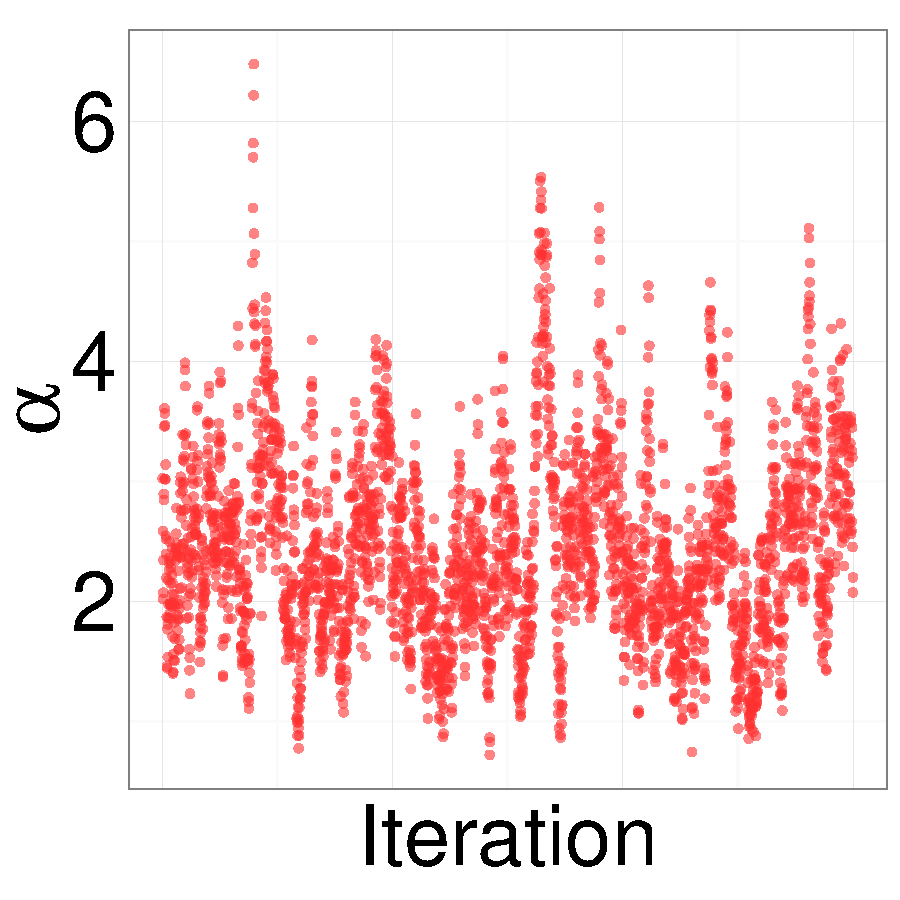
\includegraphics [width=0.24\textwidth, angle=0]{figs/QC_ks/qc_traceGBS_4_03_10_.pdf}
    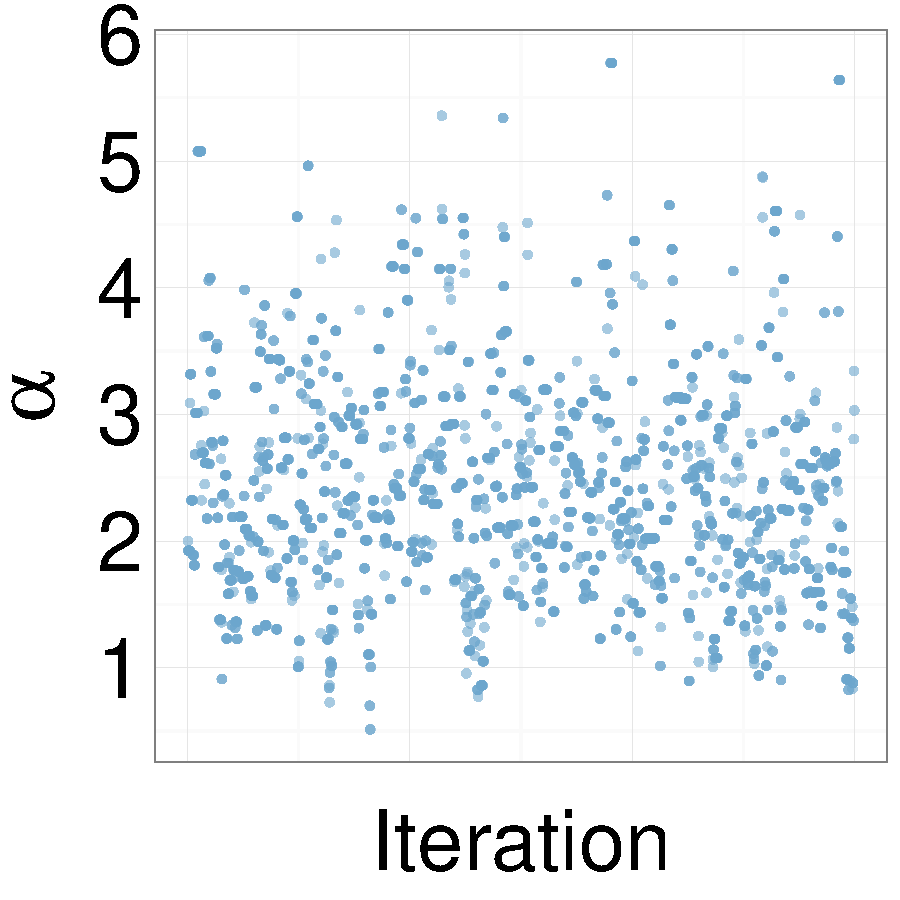
\includegraphics [width=0.24\textwidth, angle=0]{figs/QC_ks/qc_traceMH_4_03_10_.pdf}
    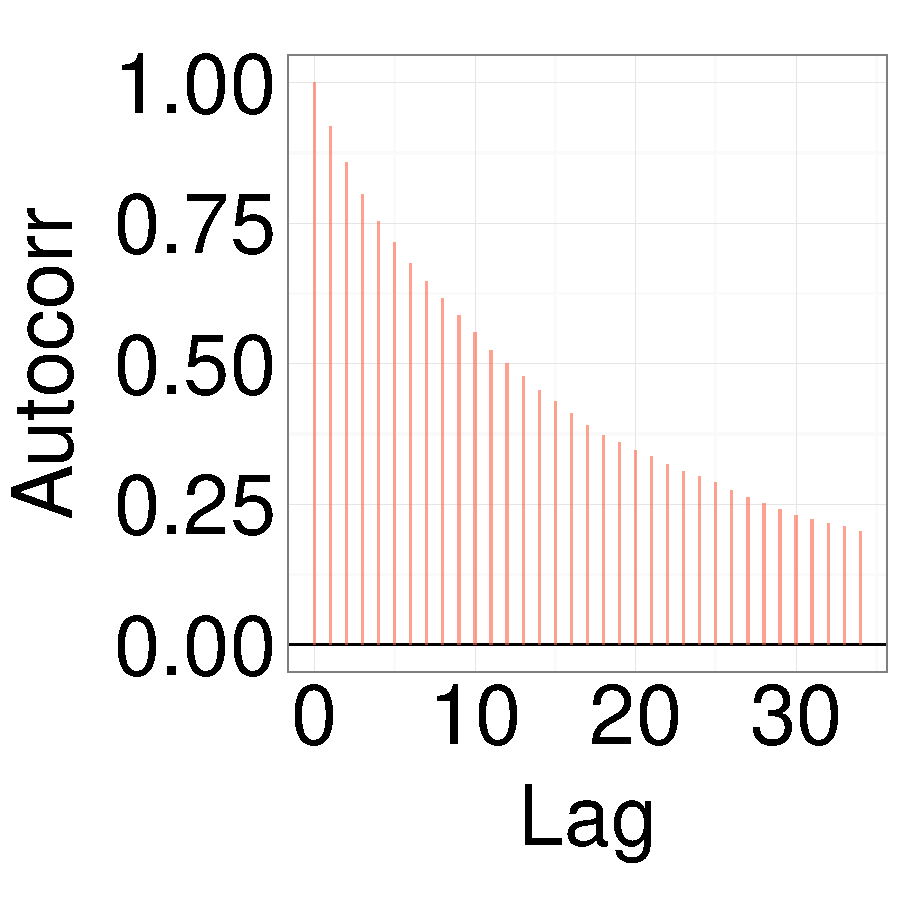
\includegraphics [width=0.24\textwidth, angle=0]{figs/QC_ks/qc_gbsacf_4_03_10_.pdf}
    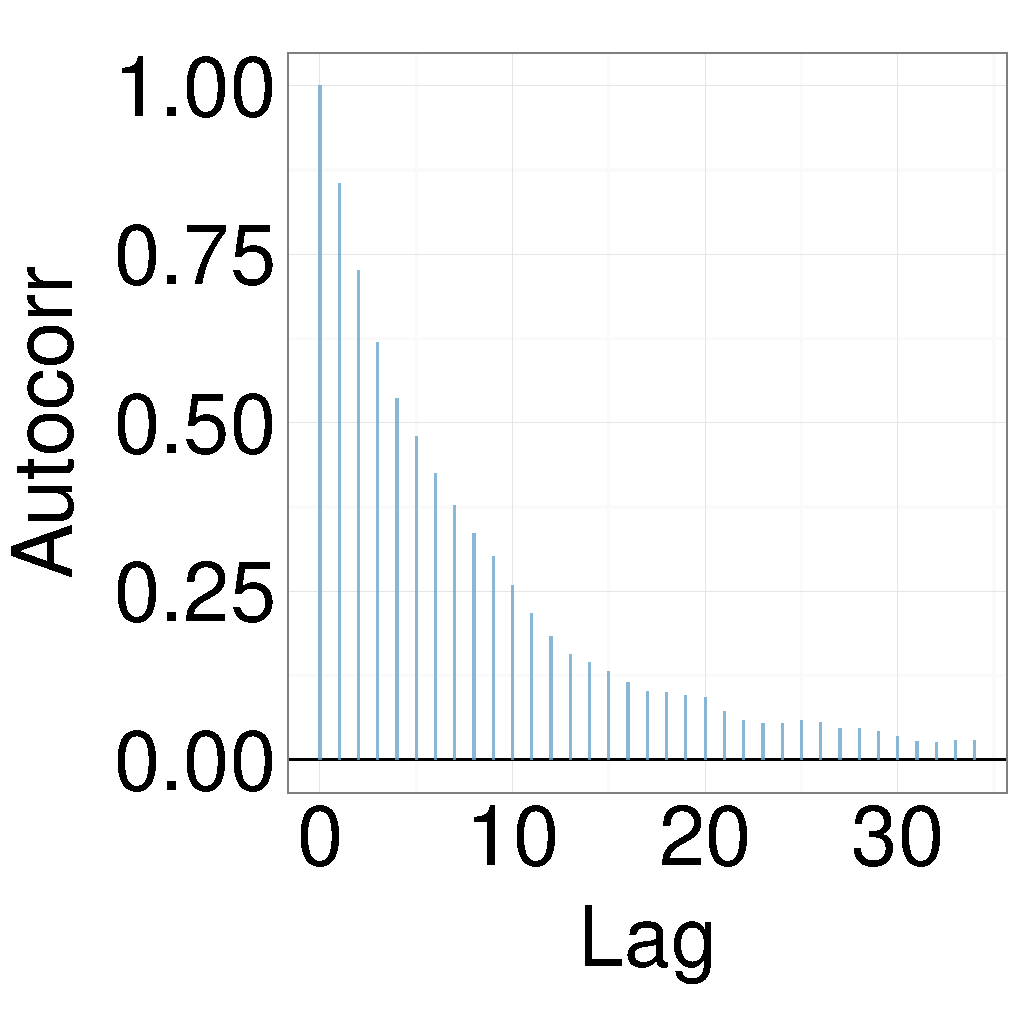
\includegraphics [width=0.24\textwidth, angle=0]{figs/QC_ks/qc_mhacf_4_03_10_.pdf}
  \end{minipage}

%  \end{minipage}
%  \begin{minipage}[!hp]{0.99\linewidth}
    \caption{The left is histogram for the posterior samples($\alpha$) of the time-inhomogeneous immigration model with dimension 10, the red and blue curves are the Gibbs and symmetrized MH. The p value of the two sample-Kolmogorov Smirnov test is $ 0.7212$. The middle and the right are trace plots for the posterior samples of the time-inhomogeneous immigration model with dimension 10, the middle is for Gibbs and the right is for symmetrized MH}
     \label{fig:TRACE_CQ}
%  \end{minipage}
  \end{figure}


  \begin{figure}[H]
  
  \begin{minipage}[hp]{0.65\linewidth}
  \centering
    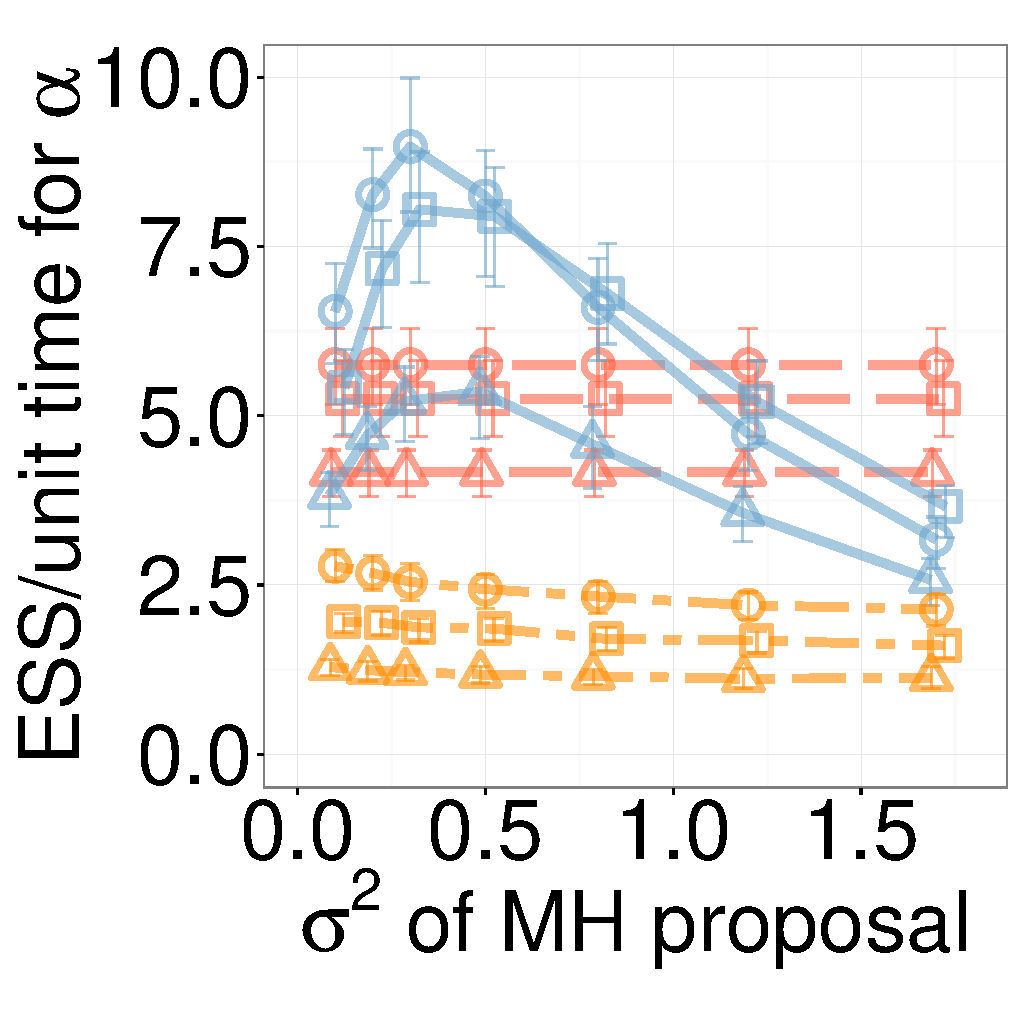
\includegraphics [width=0.44\textwidth, angle=0]{figs/new_whole_exp_figs/q_alpha_dim3.pdf}
    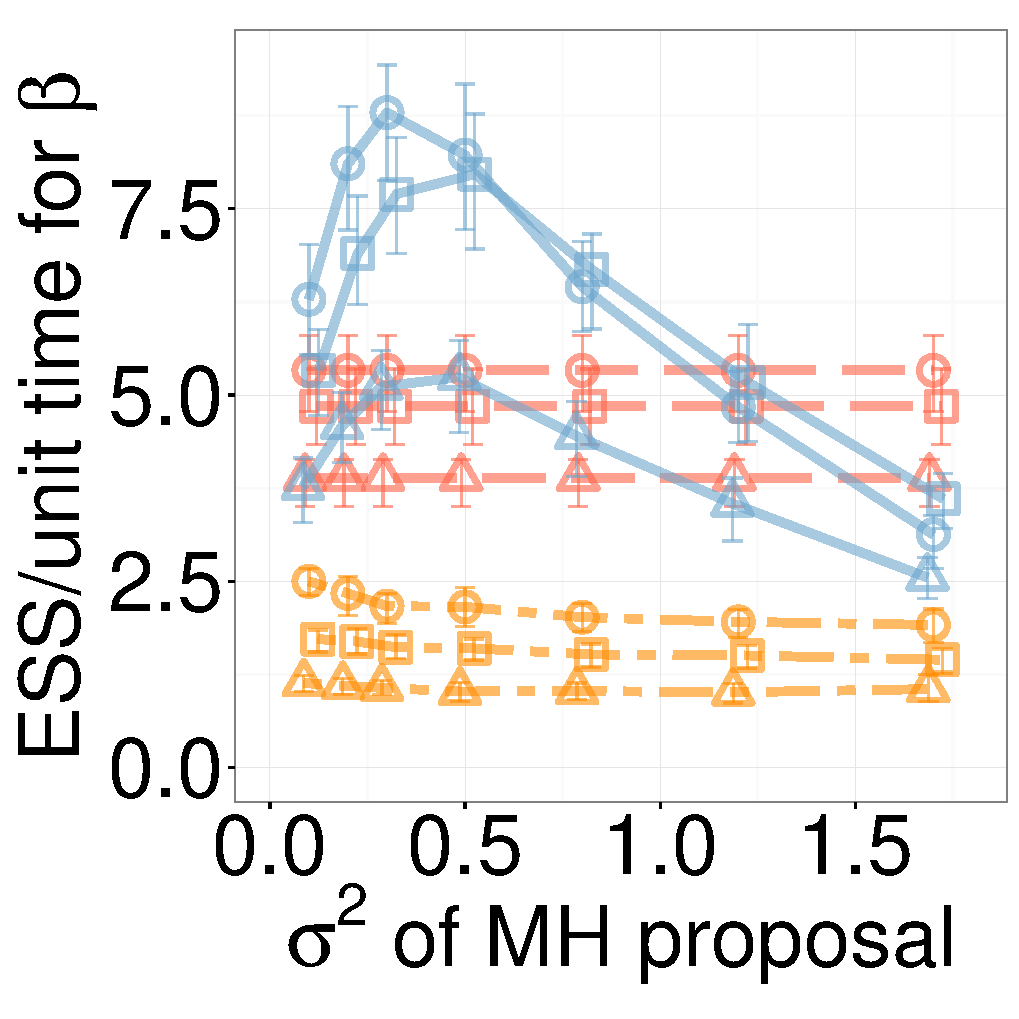
\includegraphics [width=0.44\textwidth, angle=0]{figs/new_whole_exp_figs/q_beta_dim3.pdf}
  \end{minipage}
  \begin{minipage}[!hp]{0.33\linewidth}
    \caption{ESS/sec for the immigration model, with dimension 3. (Left, 
      right) are $(\alpha, \beta)$. Blue yellow, and red curves are the symmetrized MH,
  \naive\ MH, Gibbs sampling and particle MCMC.}
     \label{fig:ESS_Q_D33}
  \end{minipage}
  \centering
  \begin{minipage}[!hp]{0.65\linewidth}
  \centering
    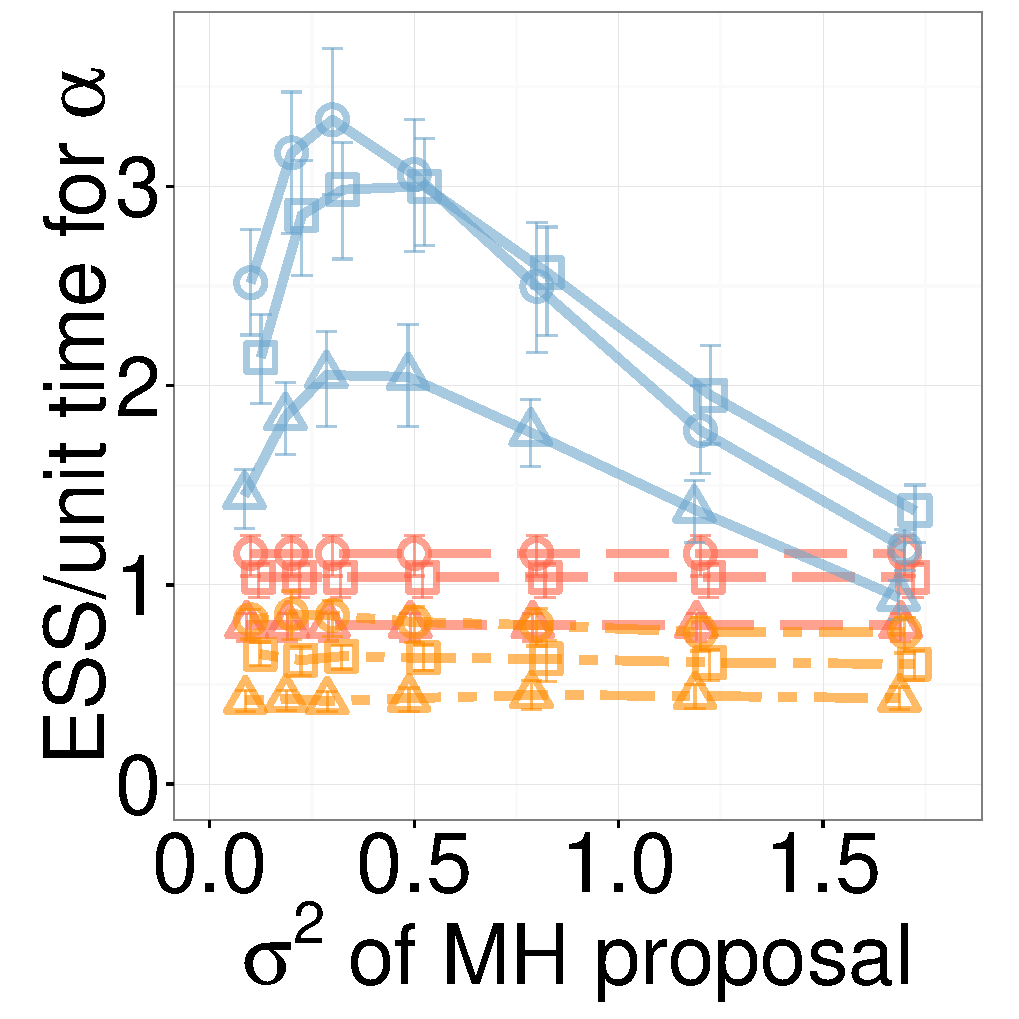
\includegraphics [width=0.44\textwidth, angle=0]{figs/new_whole_exp_figs/cq_alpha_dim3.pdf}
    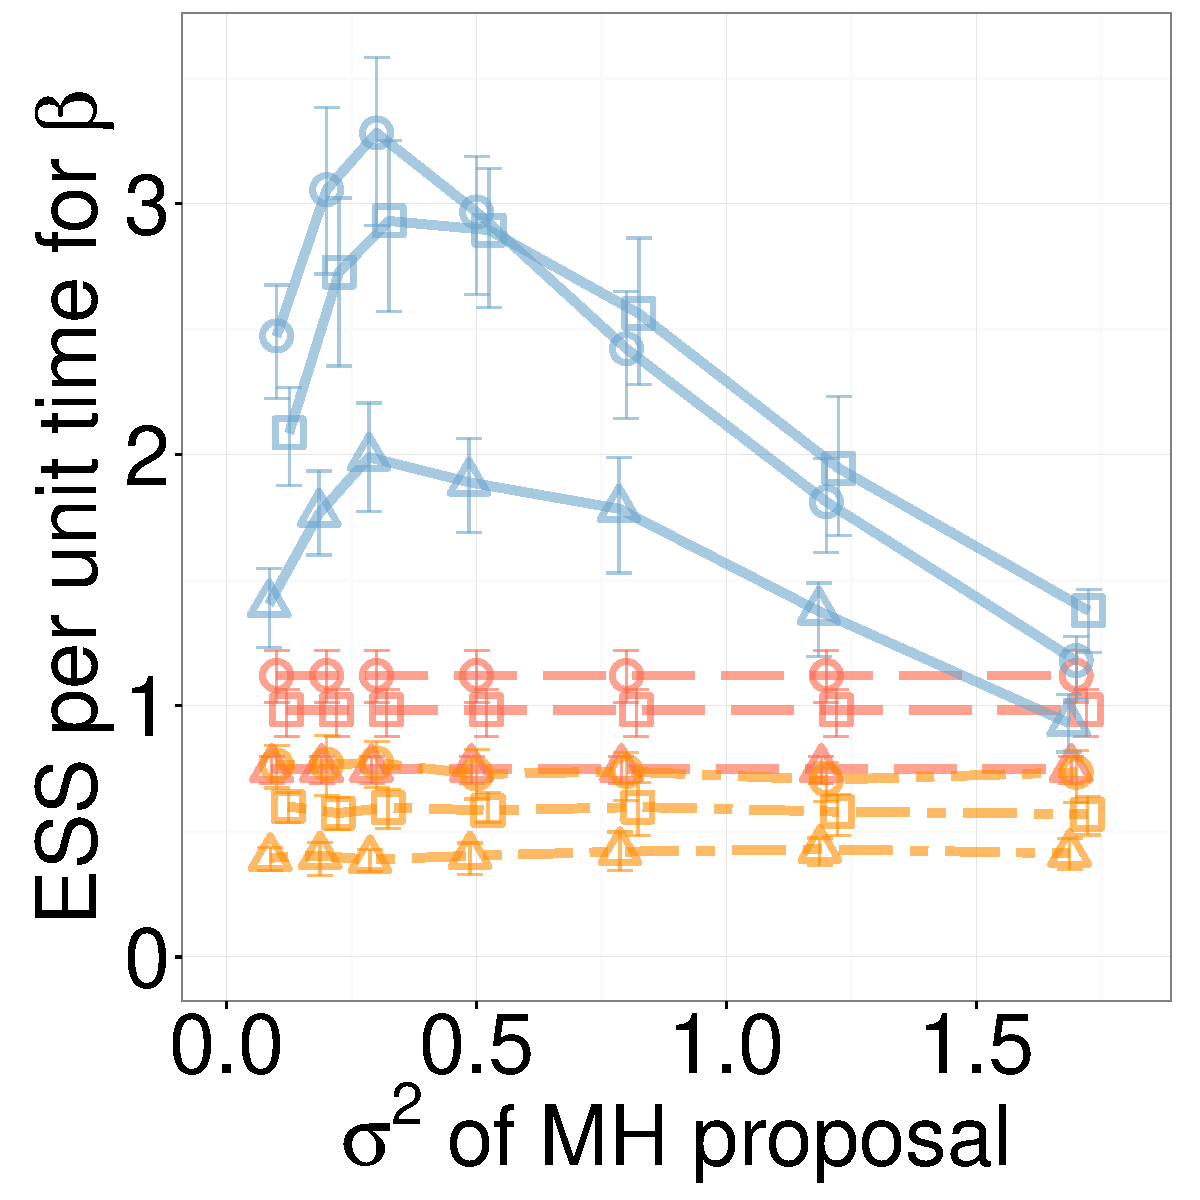
\includegraphics [width=0.44\textwidth, angle=0]{figs/new_whole_exp_figs/cq_beta_dim3.pdf}
  \end{minipage}
  \begin{minipage}[!hp]{0.33\linewidth}
    \caption{ESS/sec for the time-inhomogeneous immigration model, with 
      dimension 3. (Left, right) are $(\alpha, \beta)$. Blue, yellow and red curves are the symmetrized MH,
  \naive\ MH, and Gibbs algorithm.}
     \label{fig:ESS_pc_33}
  \end{minipage}

 \begin{minipage}[hp]{0.65\linewidth}
  \centering
    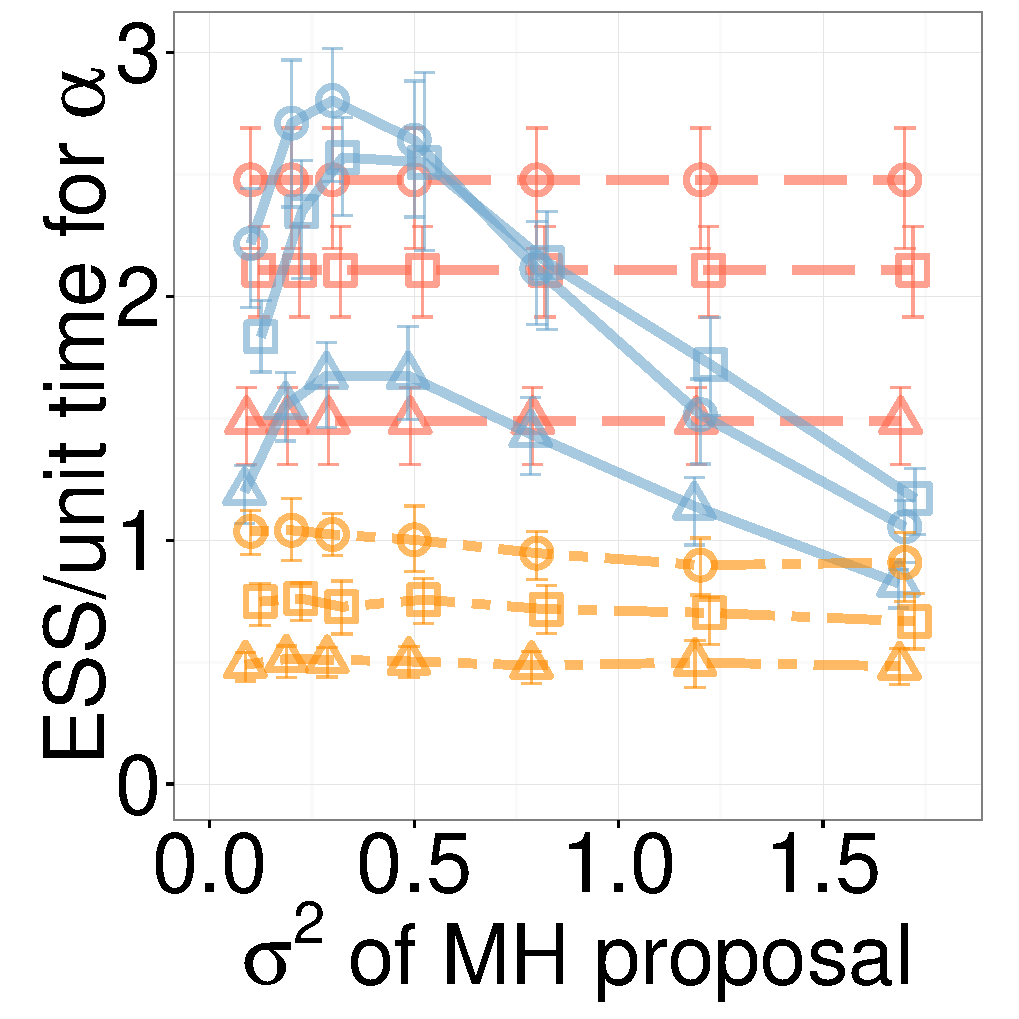
\includegraphics [width=0.44\textwidth, angle=0]{figs/new_whole_exp_figs/q_alpha_dim5.pdf}
    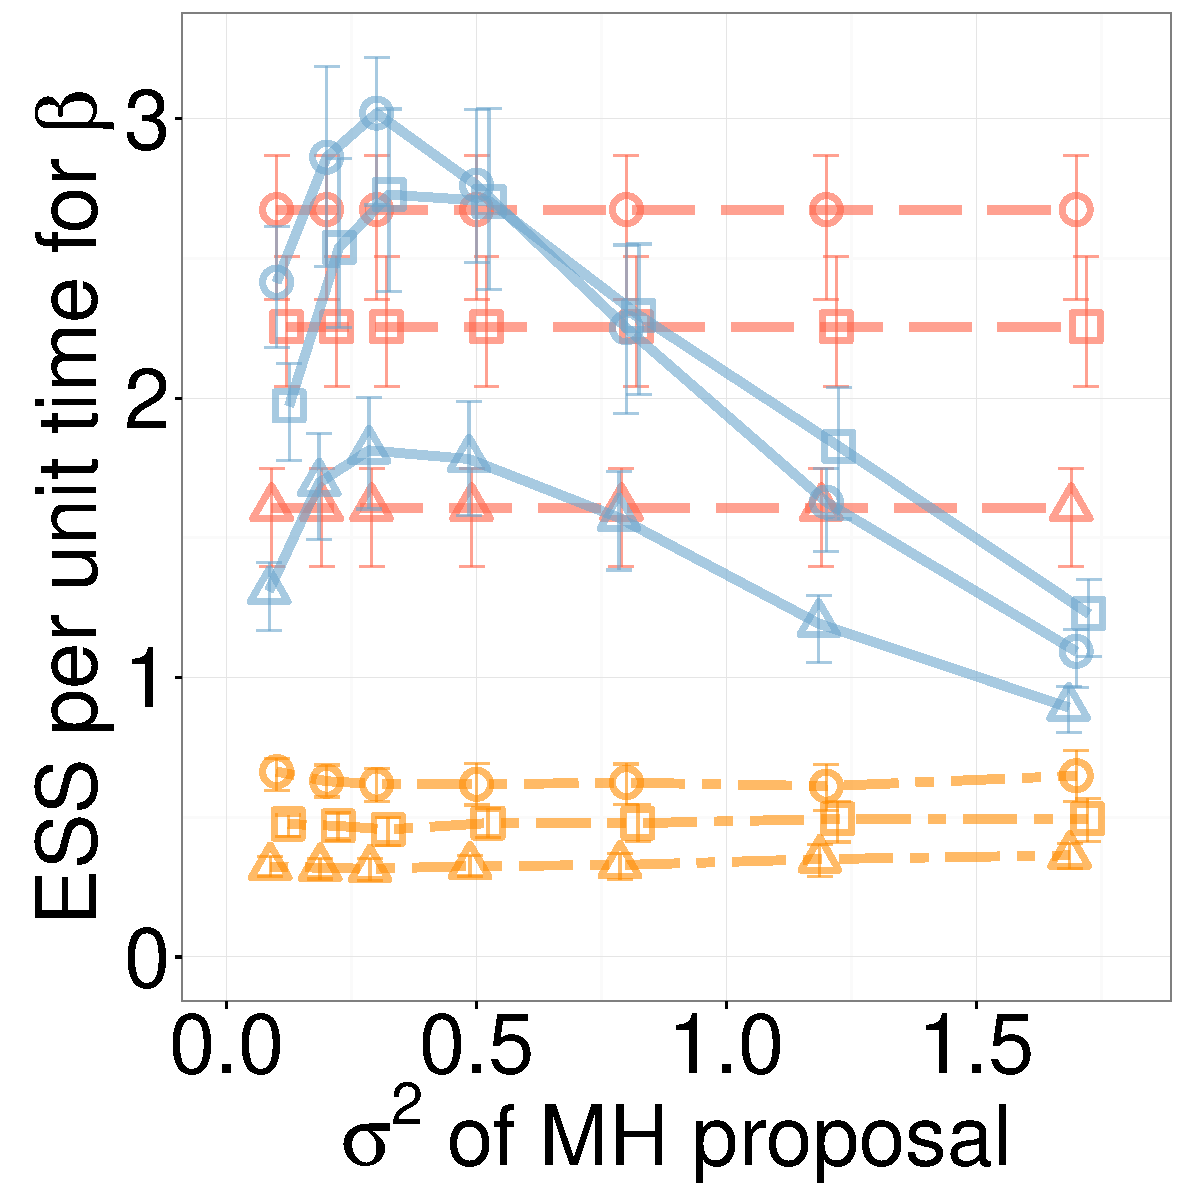
\includegraphics [width=0.44\textwidth, angle=0]{figs/new_whole_exp_figs/q_beta_dim5.pdf}
  \end{minipage}
  \begin{minipage}[!hp]{0.33\linewidth}
    \caption{ESS/sec for the immigration model, with dimension 5. (Left, 
      right) are $(\alpha, \beta)$. Red, yellow, and blue curves are the symmetrized MH,
  \naive\ MH, Gibbs sampling and particle MCMC.}
     \label{fig:ESS_Q_D55}
  \end{minipage}
  \centering
  \begin{minipage}[!hp]{0.65\linewidth}
  \centering
    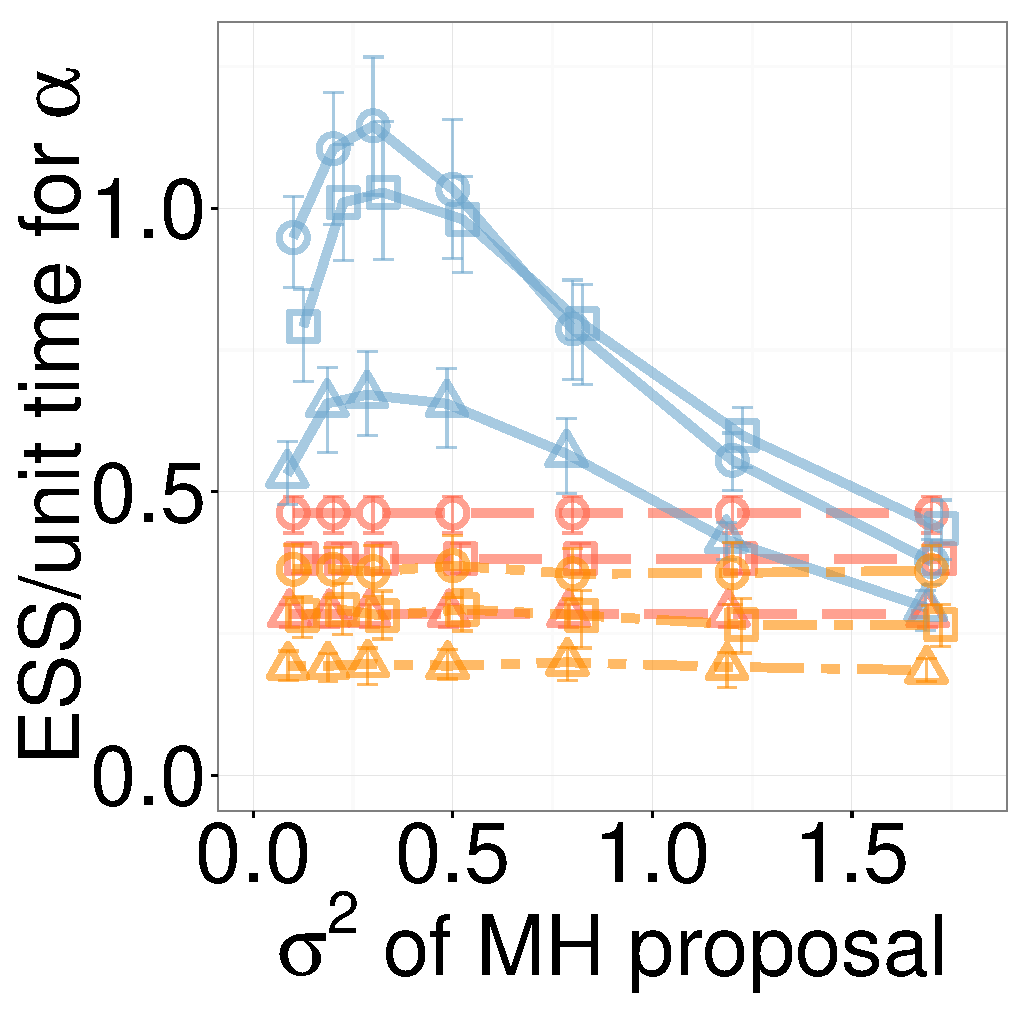
\includegraphics [width=0.44\textwidth, angle=0]{figs/new_whole_exp_figs/cq_alpha_dim5.pdf}
    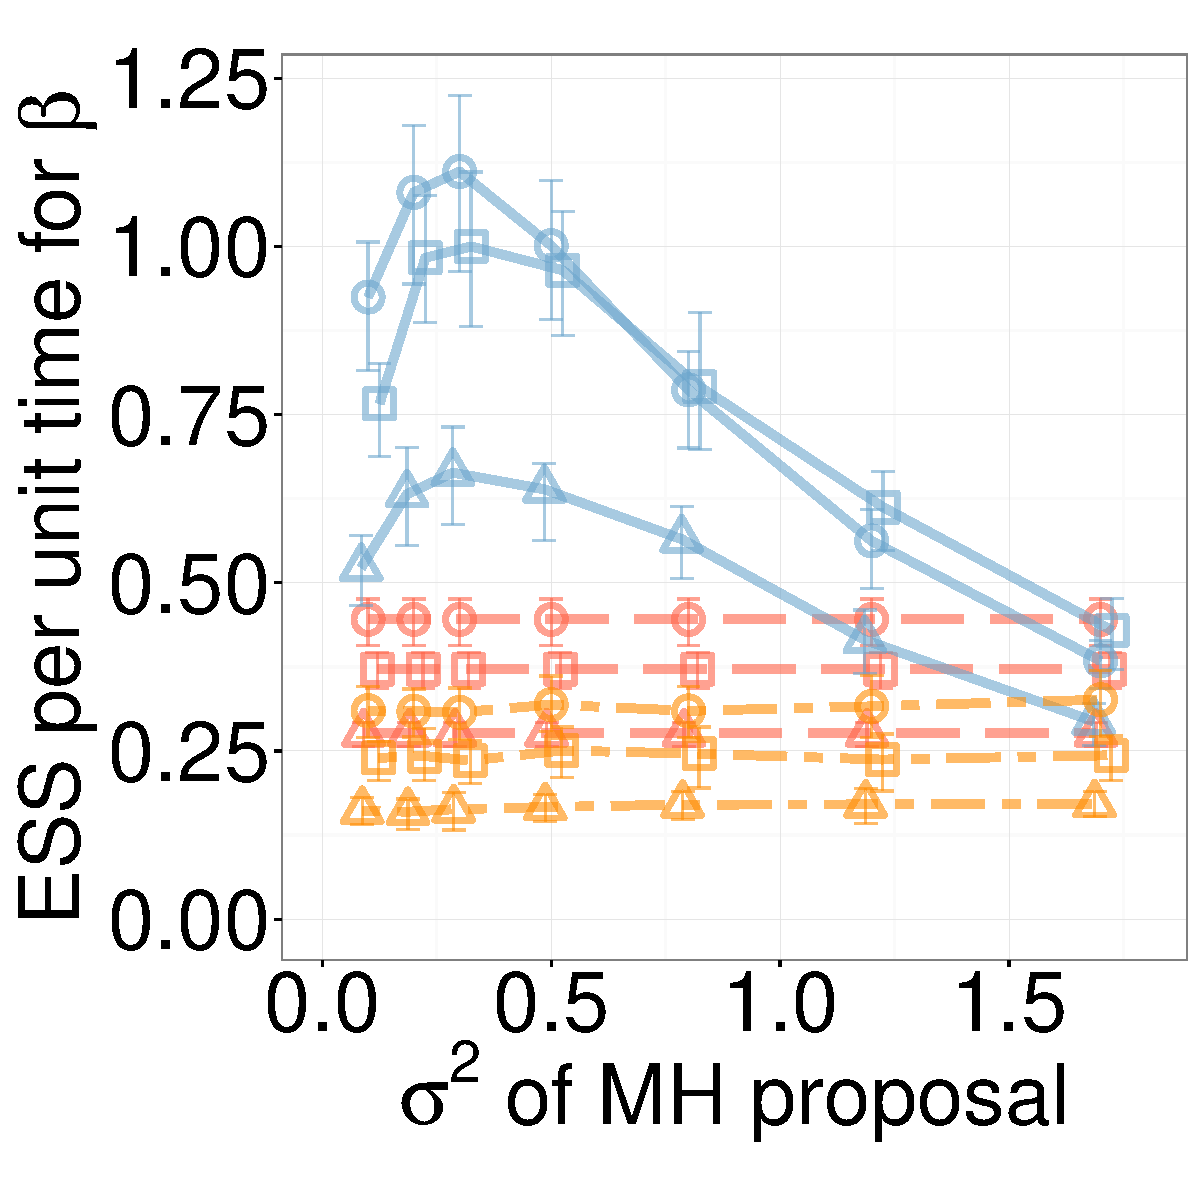
\includegraphics [width=0.44\textwidth, angle=0]{figs/new_whole_exp_figs/cq_beta_dim5.pdf}
  \end{minipage}
  \begin{minipage}[!hp]{0.33\linewidth}
    \caption{ESS/sec for the time-inhomogeneous immigration model, with 
      dimension 5. (Left, right) are $(\alpha, \beta)$. Blue, yellow and red curves are the symmetrized MH,
  \naive\ MH, and Gibbs algorithm.}
     \label{fig:ESS_pc_55}
  \end{minipage}

  \begin{minipage}[!hp]{0.65\linewidth}
  \centering
    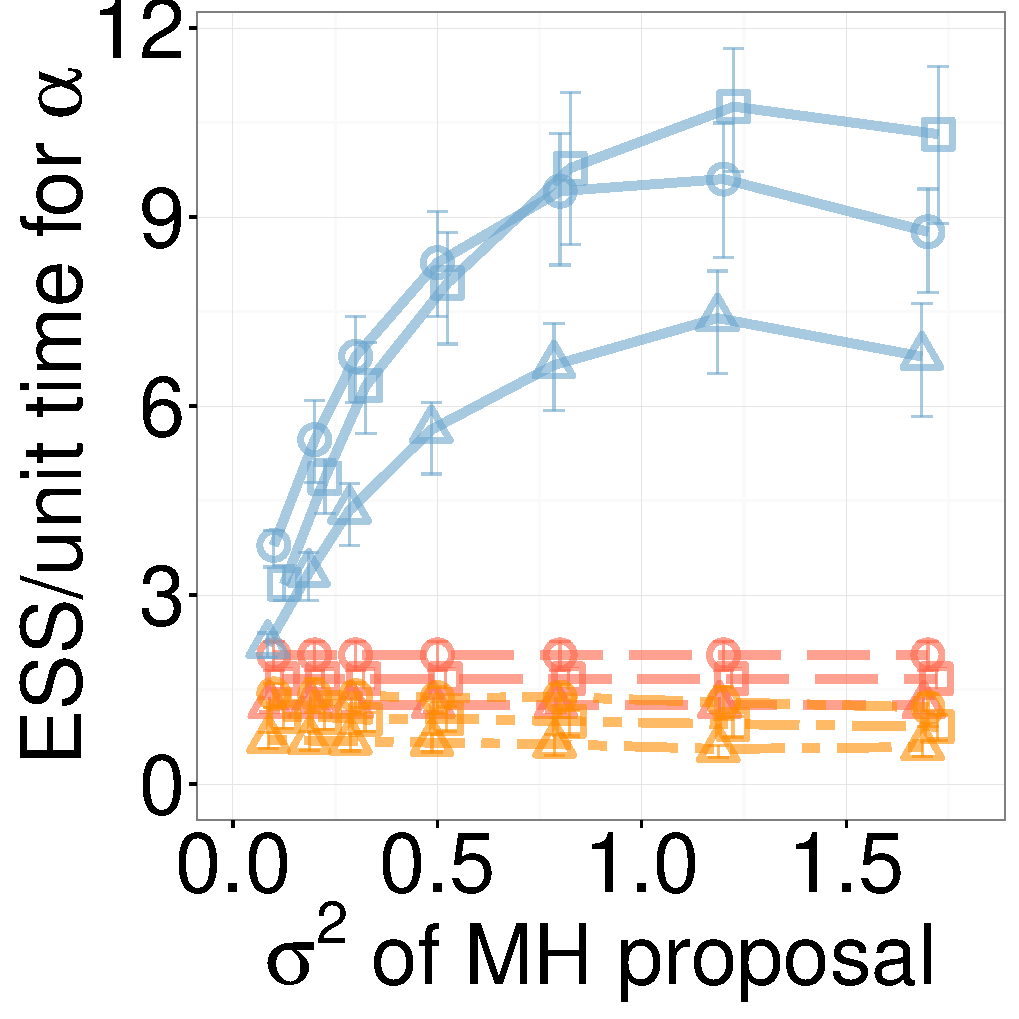
\includegraphics [width=0.44\textwidth, angle=0]{figs/new_whole_exp_figs/jc_alpha.pdf}
  \end{minipage}
  \begin{minipage}[!hp]{0.33\linewidth}
    \caption{ESS/sec for the JC immigration model, with 
      dimension 5. (Left, right) are $(\alpha, \beta)$. Blue, yellow and red curves are the symmetrized MH,
  \naive\ MH, and Gibbs algorithm.}
     \label{fig:ESS_pc_55}
  \end{minipage}

 \begin{minipage}[hp]{0.65\linewidth}
  \centering
    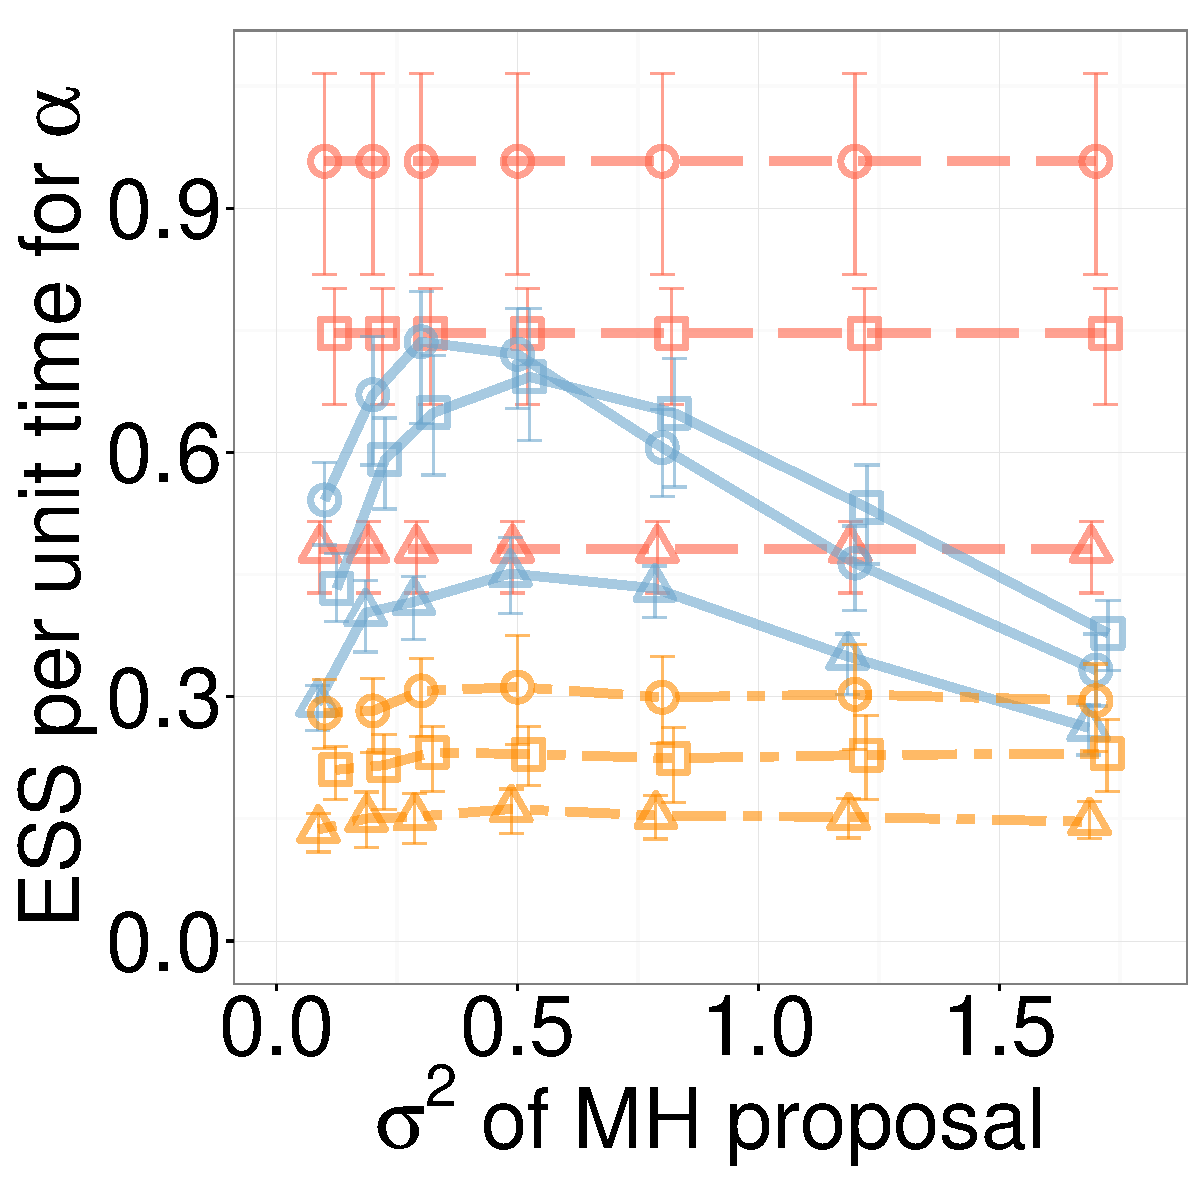
\includegraphics [width=0.44\textwidth, angle=0]{figs/new_whole_exp_figs/q_alpha_dim10.pdf}
    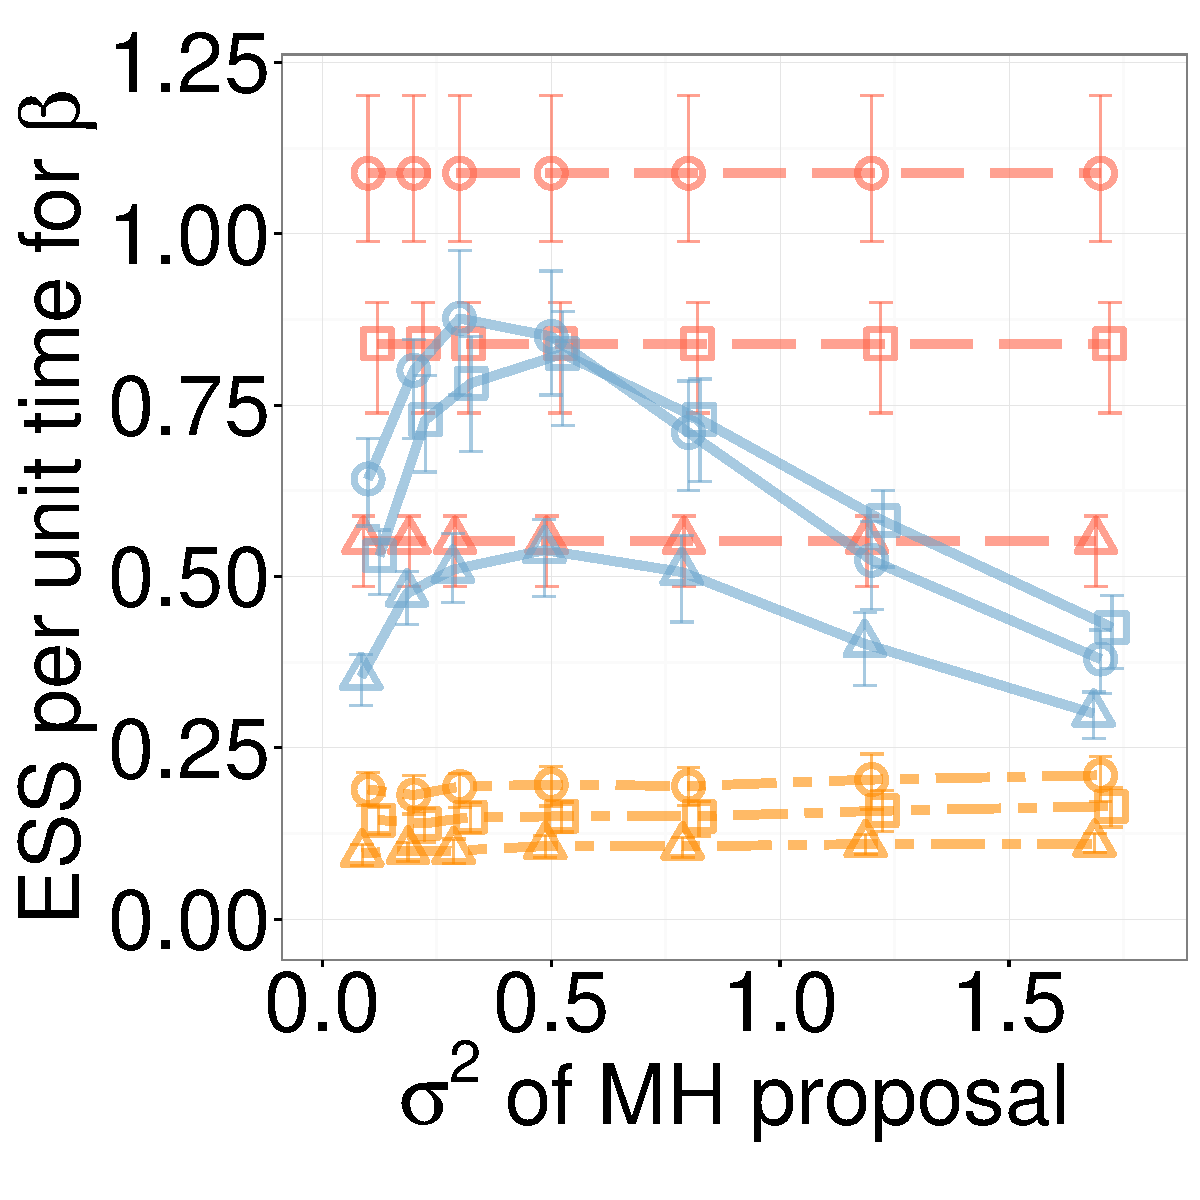
\includegraphics [width=0.44\textwidth, angle=0]{figs/new_whole_exp_figs/q_beta_dim10.pdf}
  \end{minipage}
  \begin{minipage}[!hp]{0.33\linewidth}
    \caption{ESS/sec for the immigration model, with dimension 5. (Left, 
      right) are $(\alpha, \beta)$. Blue, yellow, and red curves are the symmetrized MH,
  \naive\ MH, Gibbs sampling and particle MCMC.}
     \label{fig:ESS_Q_D1010}
  \end{minipage}
  \centering
  \begin{minipage}[!hp]{0.65\linewidth}
  \centering
    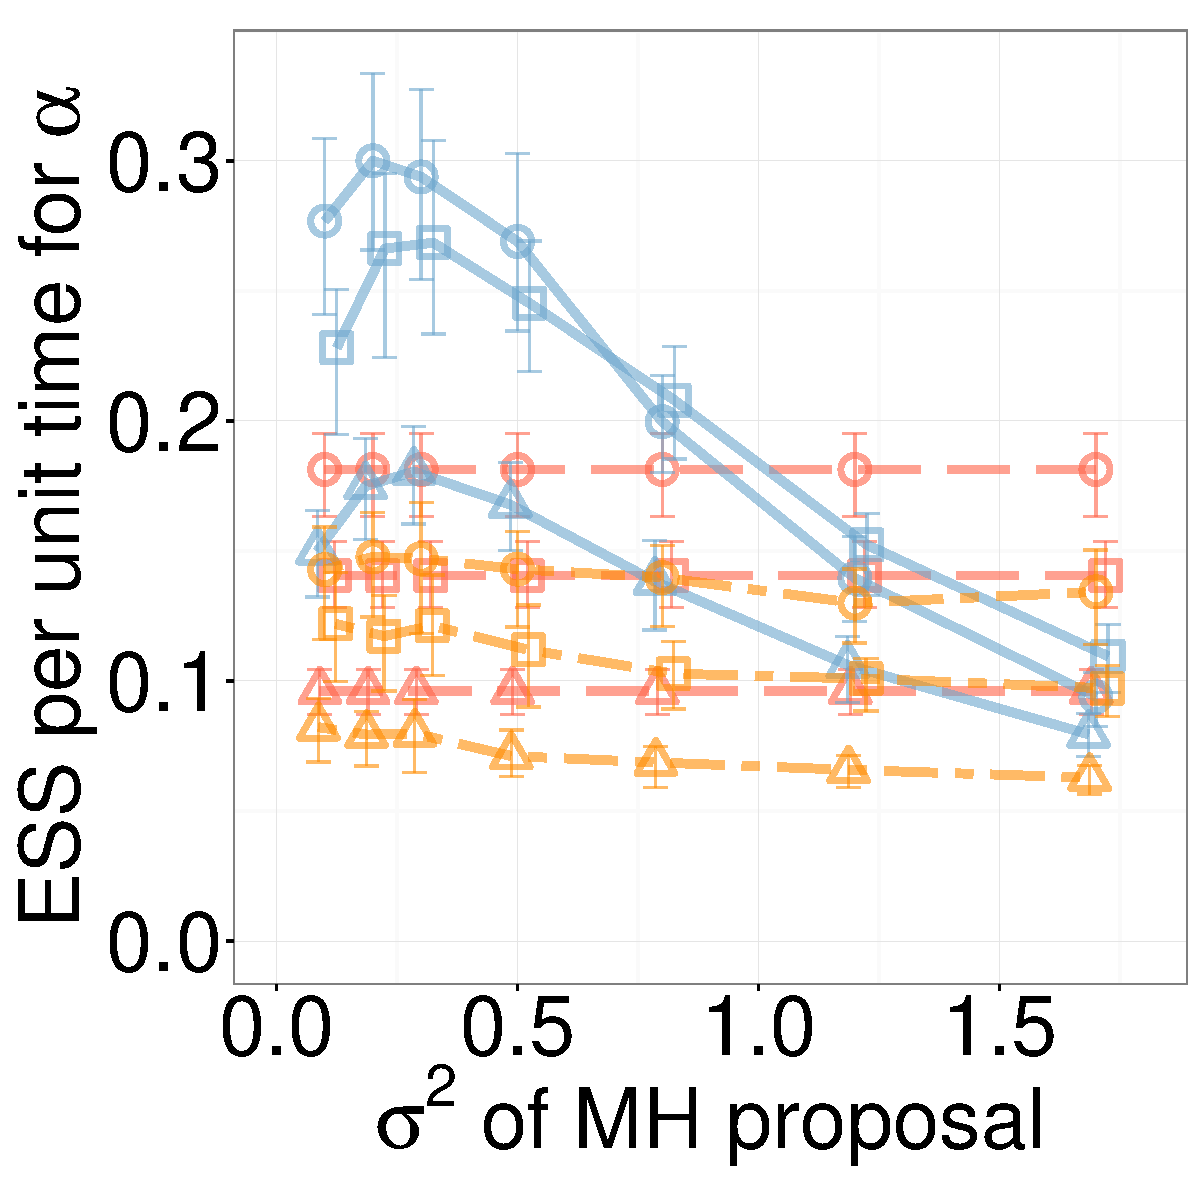
\includegraphics [width=0.44\textwidth, angle=0]{figs/new_whole_exp_figs/cq_alpha_dim10.pdf}
    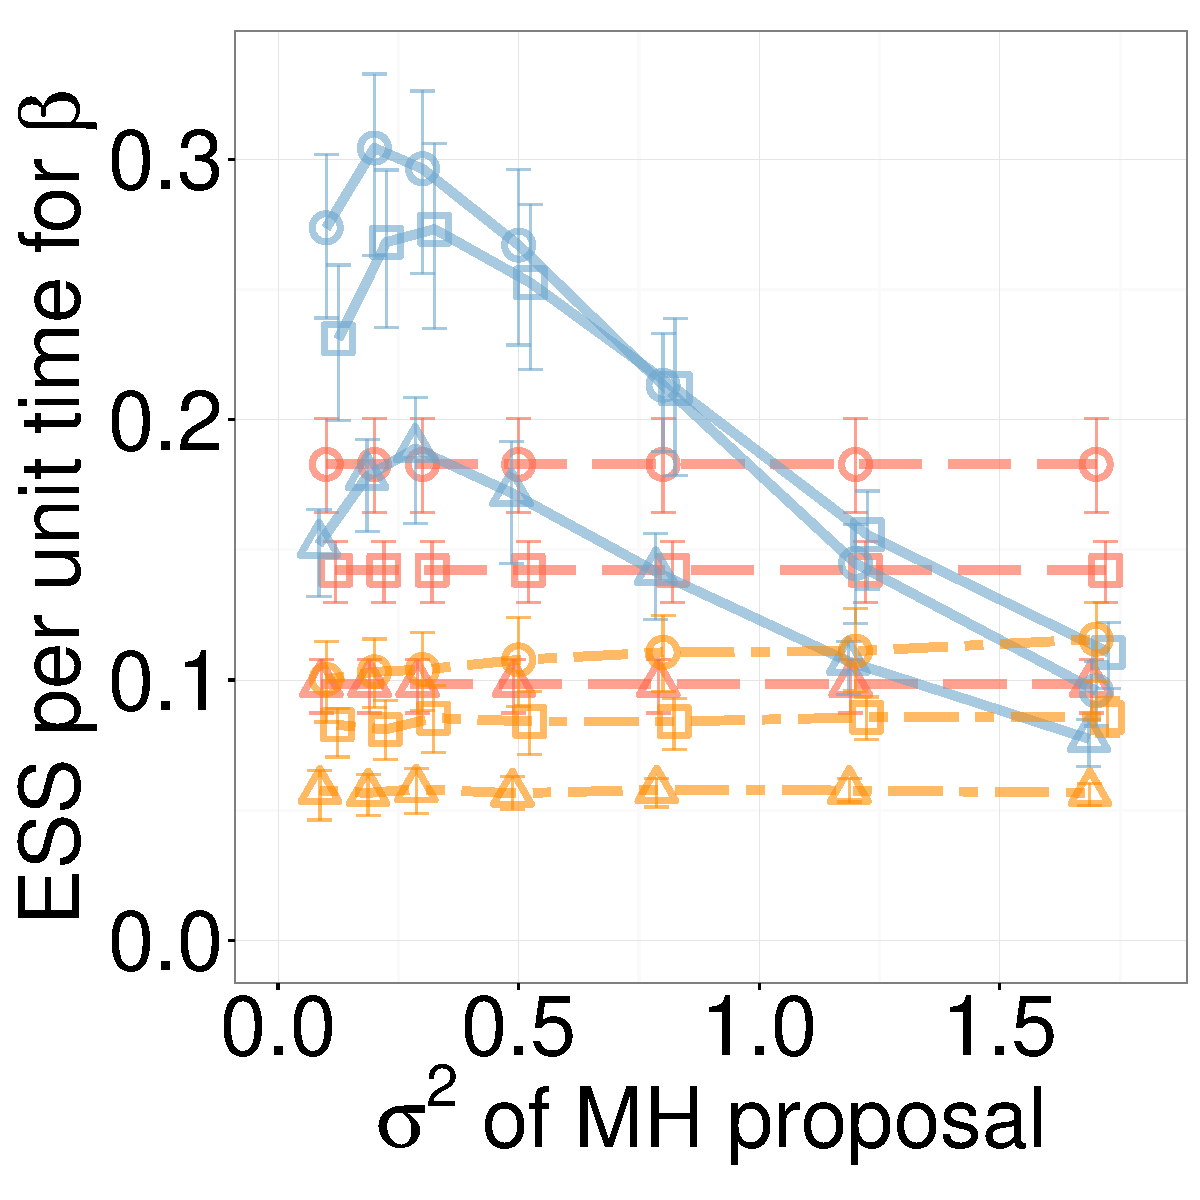
\includegraphics [width=0.44\textwidth, angle=0]{figs/new_whole_exp_figs/cq_beta_dim10.pdf}
  \end{minipage}
  \begin{minipage}[!hp]{0.33\linewidth}
    \caption{ESS/sec for the time-inhomogeneous immigration model, with 
      dimension 5. (Left, right) are $(\alpha, \beta)$. Blue, yellow and red curves are the symmetrized MH,
  \naive\ MH, and Gibbs algorithm.}
     \label{fig:ESS_pc_1010}
  \end{minipage}

% \centering
% \begin{minipage}[!hp]{0.64\linewidth}
%   \hspace{.15in}
%   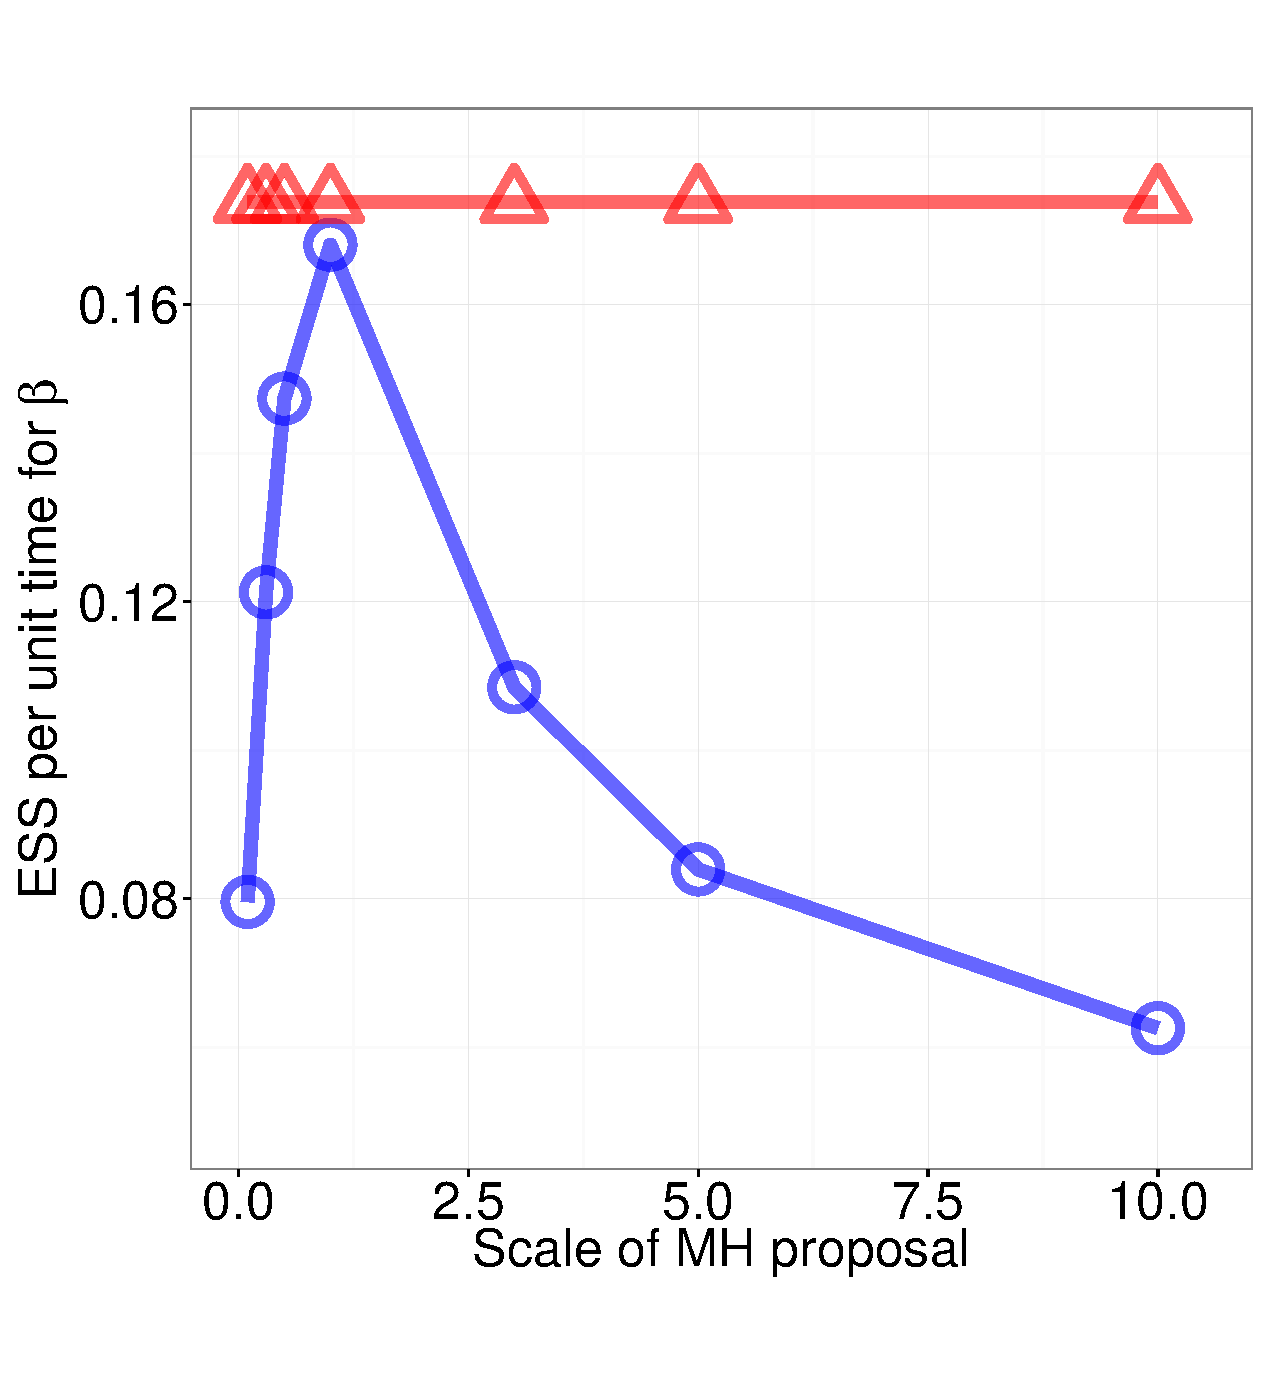
\includegraphics [width=0.44\textwidth, angle=0]{figs/ECOLI_beta.pdf}
%   \hspace{.15in}
%   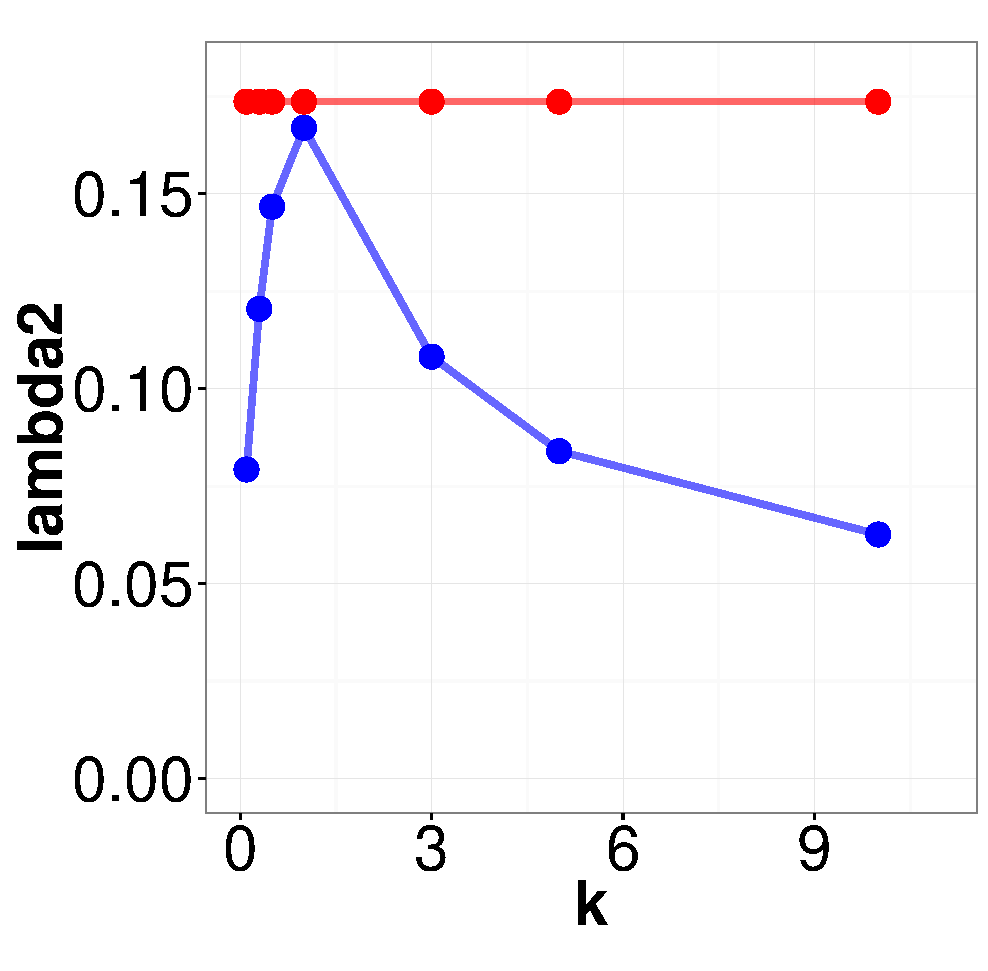
\includegraphics [width=0.44\textwidth, angle=0]{figs/ECOLI_l2.pdf}
% \end{minipage}
%   \hspace{-.3in}
% \begin{minipage}[!hp]{0.05\linewidth}
%   \hspace{0in}
%   \end{minipage}
% \begin{minipage}[!hp]{0.33\linewidth}
%   \caption{ESS/sec for EColi data. The left column is for $\beta$, and the 
%   right is for $\lambda_2$. Red and blue curves are Gibbs algorithm and the symmetrized MH.}
% \end{minipage}
%    \label{fig:ECOLI_beta_l2}
  \end{figure}
  \begin{figure}[H]
%    \vspace{-.2in}
  \centering

  \begin{minipage}[!hp]{0.99\linewidth}
    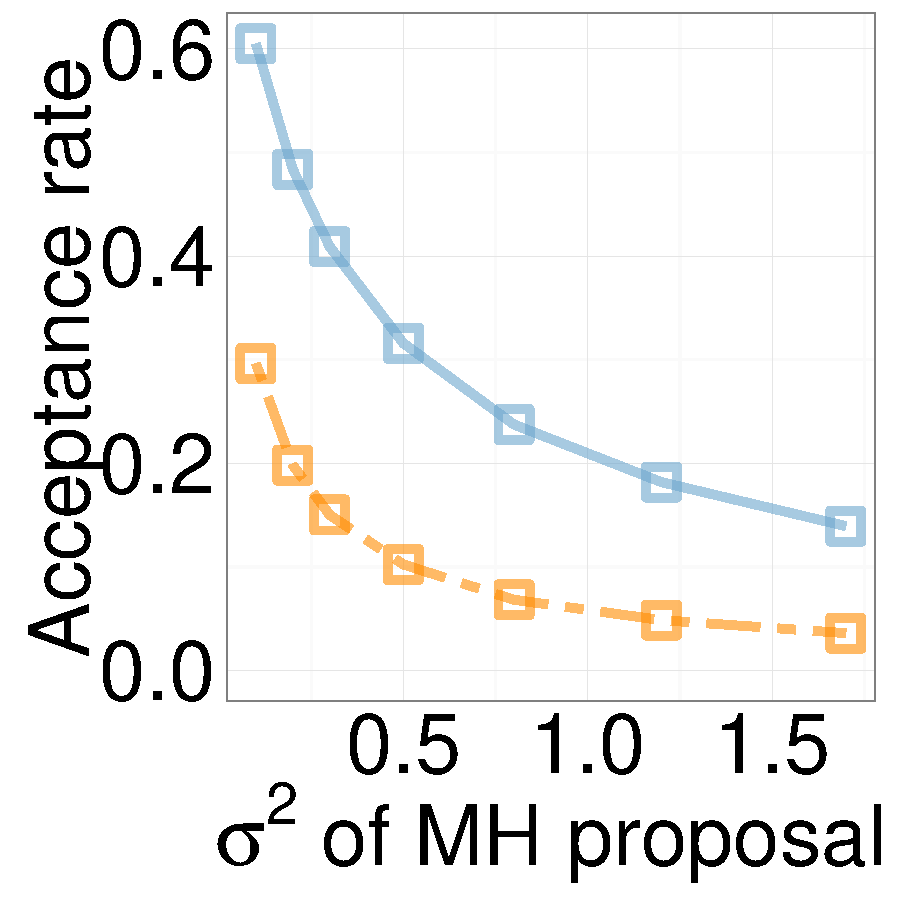
\includegraphics [width=0.40\textwidth, angle=0]{figs/acc/Q_D3alpha_k2.pdf}
	\hspace{.5in}
    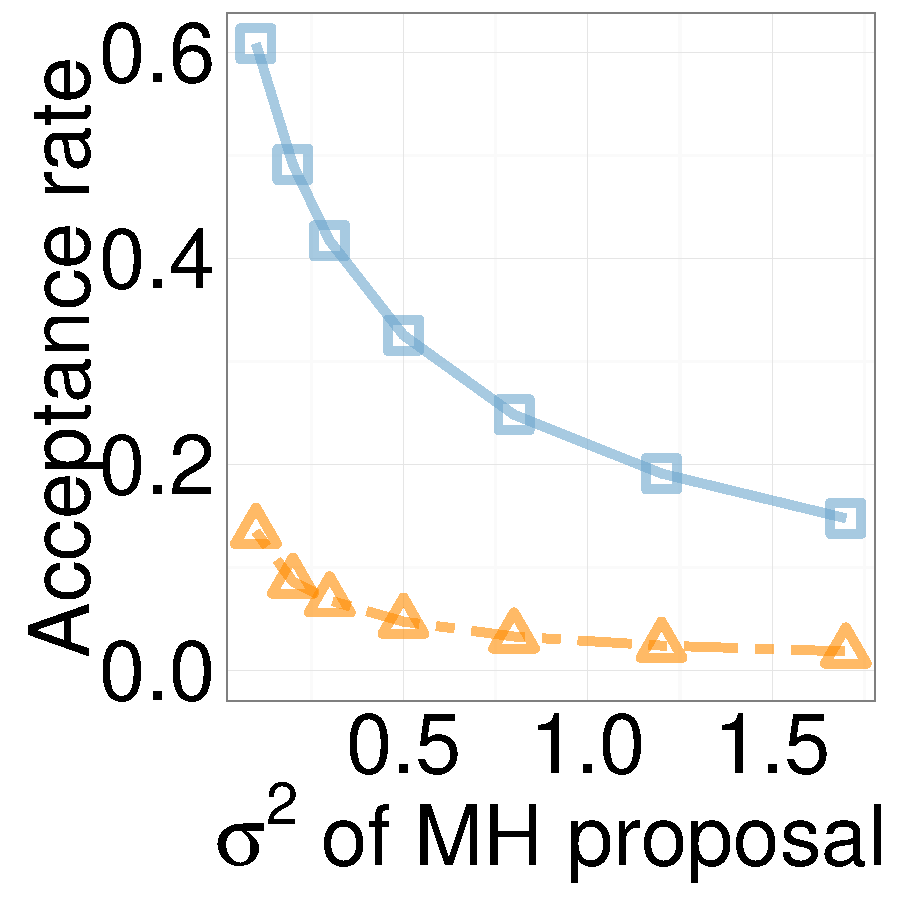
\includegraphics [width=0.40\textwidth, angle=0]{figs/acc/Q_D10alpha_k2.pdf}
  \end{minipage}
%  \begin{minipage}[!hp]{0.99\linewidth}
    \caption{Acceptance Rate for $\alpha$ in the synthetic model, the left row being dimension 3, and the right,dimension 10.  Yellow and blue curves represent symmetrized MH,
 and \naive\ MH  algorithm. The multiplicative factor is $2$. }
     \label{fig:ACC_Q}
%  \end{minipage}
  \end{figure}

%%%% Time-homog
%    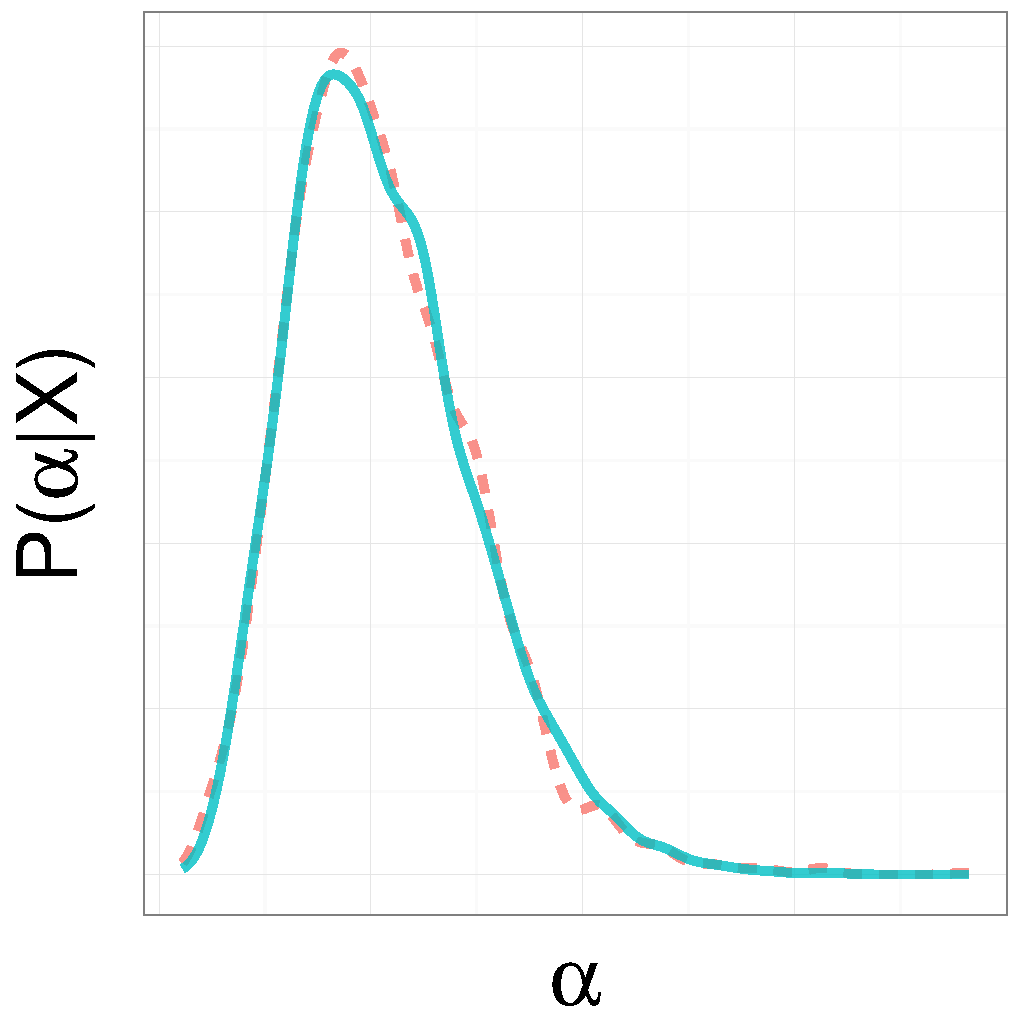
\includegraphics [width=0.19\textwidth, angle=0]{figs/Q_ks/q_hist_20_03_3_.pdf}
%%%%%%%%

  \begin{figure}[H]
%    \vspace{-.2in}
  \centering

  \begin{minipage}[!hp]{0.99\linewidth}
    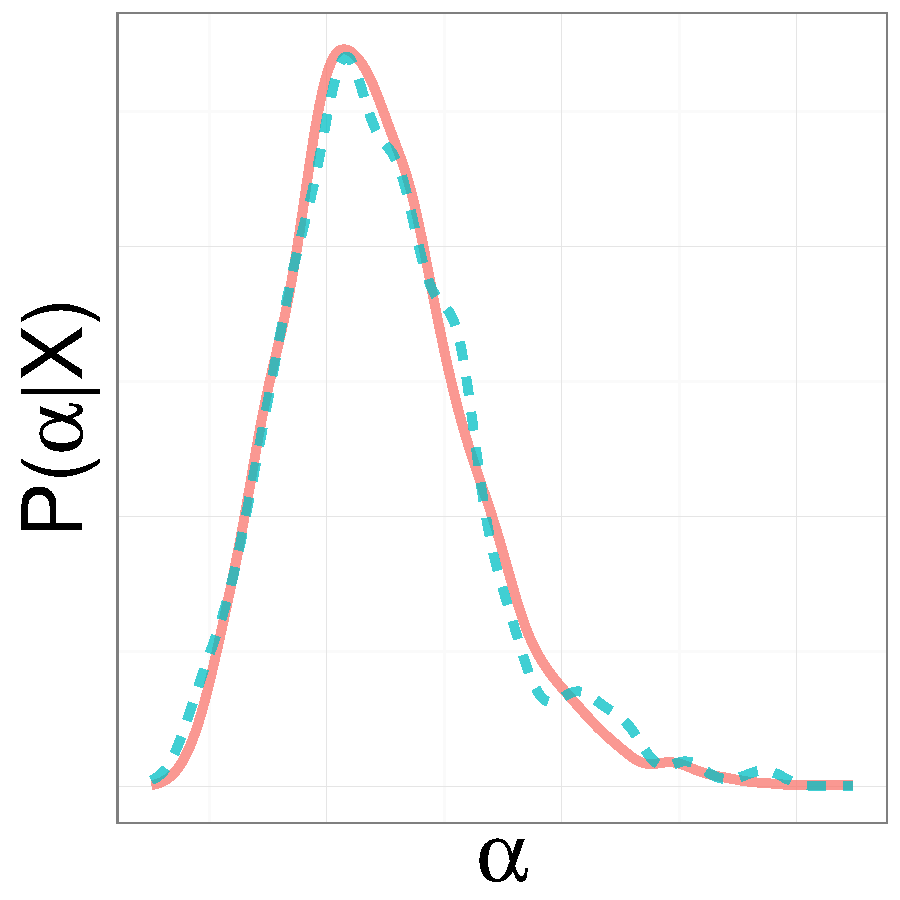
\includegraphics [width=0.3\textwidth, angle=0]{figs/QC_ks/qc_hist_4_03_10_.pdf}
    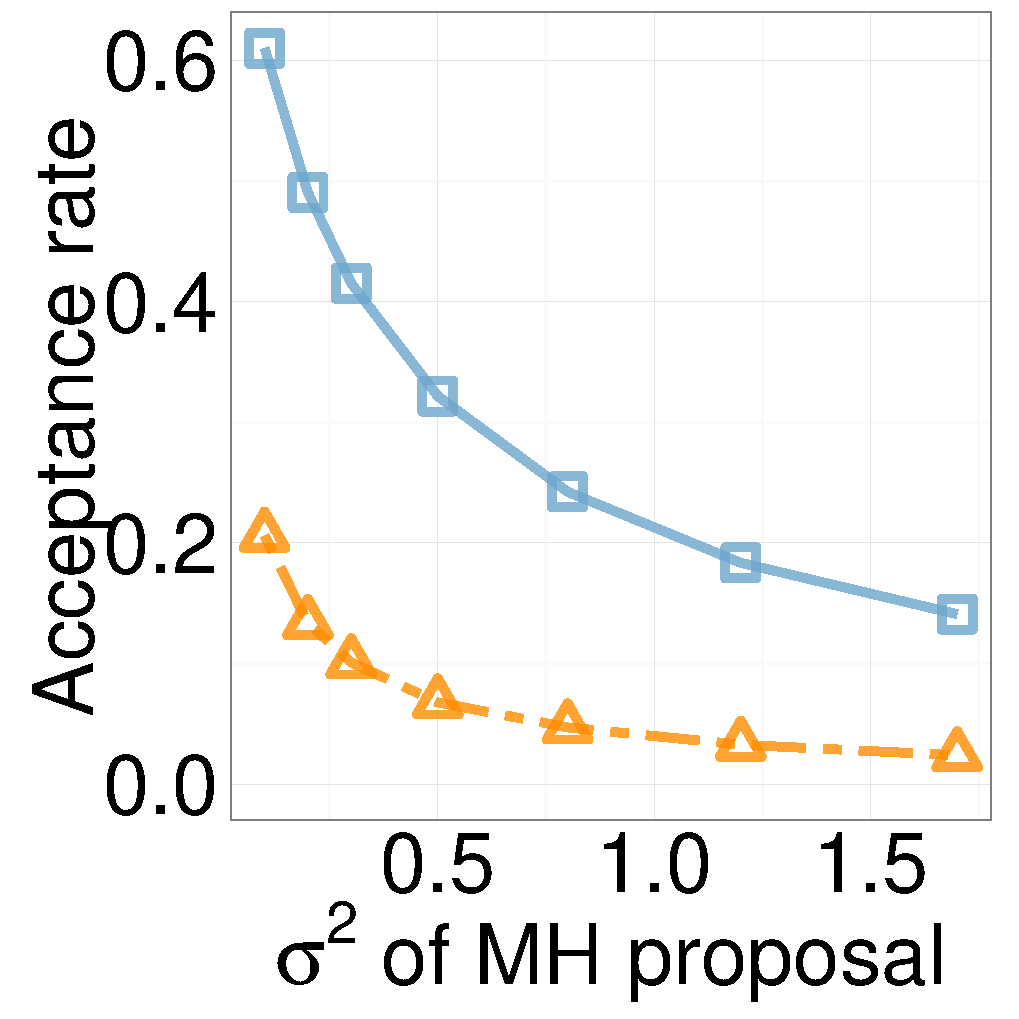
\includegraphics [width=0.30\textwidth, angle=0]{figs/acc/CQ_D3alpha_k2.pdf}
	\hspace{.5in}
    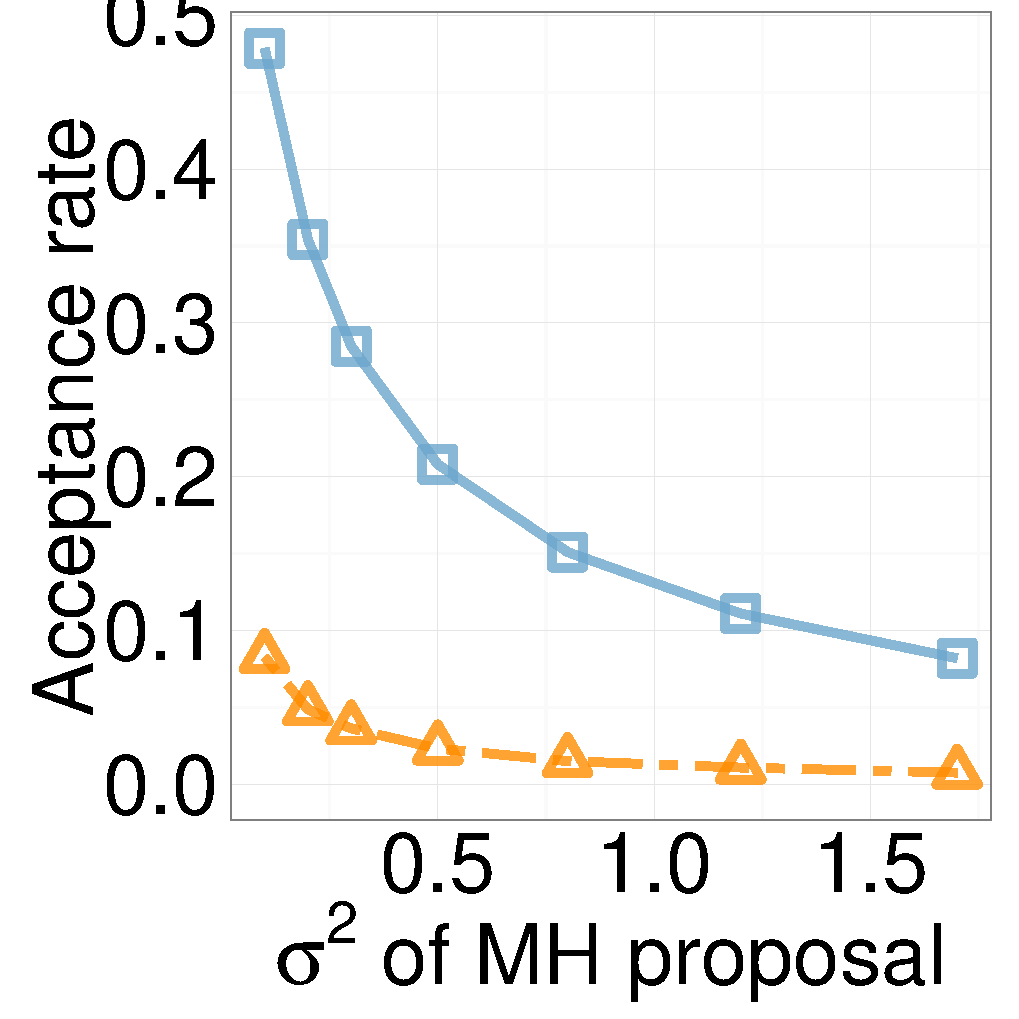
\includegraphics [width=0.30\textwidth, angle=0]{figs/acc/CQ_D10alpha_k2.pdf}
  \end{minipage}
%  \begin{minipage}[!hp]{0.99\linewidth}
    \caption{Acceptance Rate for $\alpha$ in the time-inhomogeneous immigration model, the left row being dimension 3, and the right,dimension 10.  Yellow and blue curves represent symmetrized MH,
 and \naive\ MH  algorithm. The multiplicative factor is $2$. }
     \label{fig:ACC_CQ}
%  \end{minipage}
  \end{figure}

  \begin{figure}[H]
%    \vspace{-.2in}
  \centering

  \begin{minipage}[!hp]{0.99\linewidth}
	\centering
    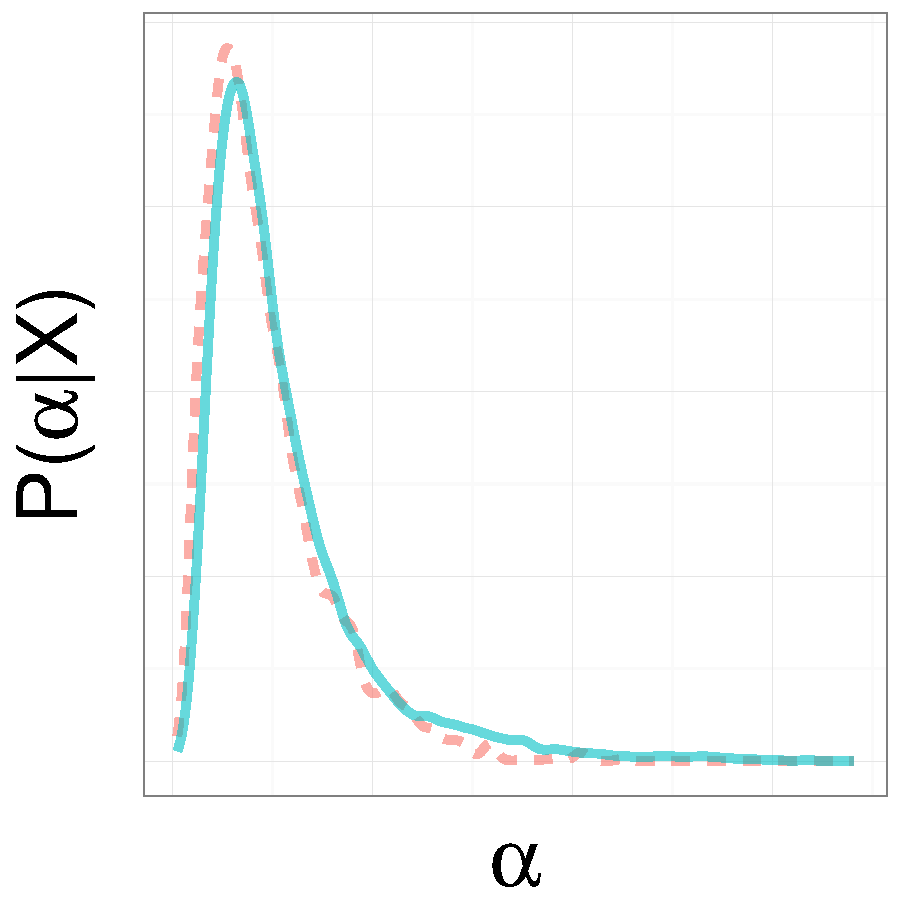
\includegraphics [width=0.3\textwidth, angle=0]{figs/ecoli_ks/ecoli_alphahist_31_3_0_.pdf}
    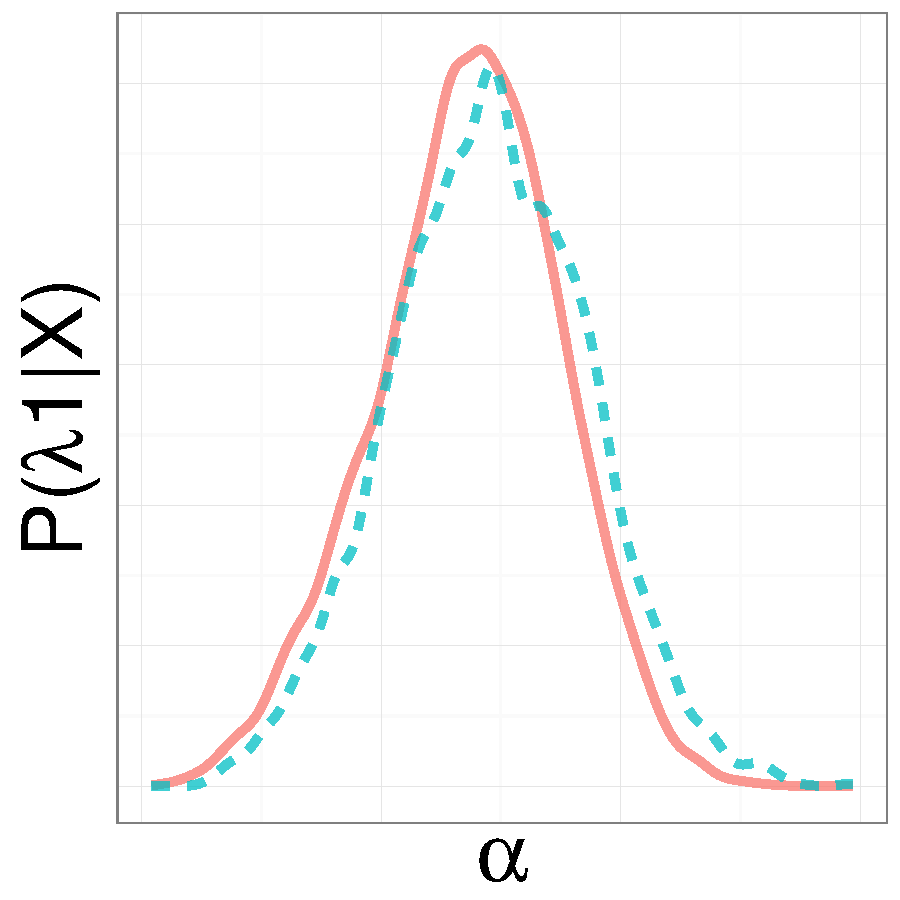
\includegraphics [width=0.3\textwidth, angle=0]{figs/ecoli_ks/ecoli_l1hist_31_3_0_.pdf}
    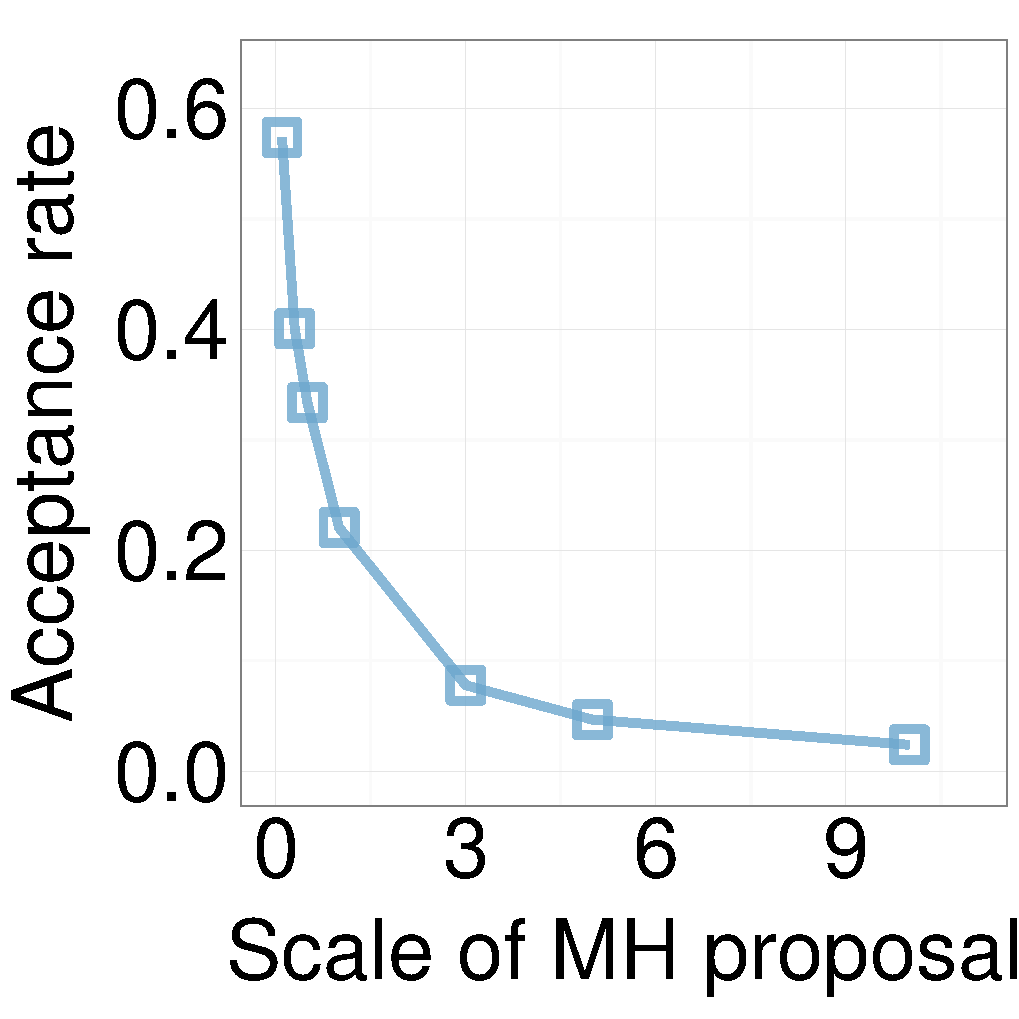
\includegraphics [width=0.30\textwidth, angle=0]{figs/acc/ecolialpha_k2.pdf}
  \end{minipage}
%  \begin{minipage}[!hp]{0.99\linewidth}
    \caption{Acceptance Rate of $\alpha$ generated by the symmetrized MH algorithm for the E.\ Coli data . The multiplicative factor is $2$. }
     \label{fig:ACC_ECOLI}
%  \end{minipage}
  \end{figure}
